% !TeX root = ../main.tex

\chapter{用户身份识别与溯源系统设计与实现}
\label{NIDTGA}

  \section{本章引言}
  \label{NIDTGA:introduction}
  NIDTGA地址生成方案\cite{liu2015building}作为一种致力于对用户身份进行溯源的IPv6地址生成技术,通过向IPv6地址接口标识中嵌入用户的网络身份标识NID与时间信息,能够减轻用户身份管理的复杂性,避免用户身份绑定信息的存储开销,并对管理域内用户的恶意上网行为产生有力的威慑作用。为了生成NIDTGA地址,需要首先获取用户身份,因此必须与网络中具体的认证手段相结合,而NIDTGA地址生成方案仅描绘了IPv6地址生成方案的蓝图,并未提出任何使用NIDTGA方案生成并配置地址的用户身份识别与溯源系统设计。事实上,由于实际的接入网络环境错综复杂,有线网络与无线网络组网方式有别,IPv6地址配置方式多种多样,用户接入认证手段迥异,而NIDTGA地址承载用户身份的能力将用户认证与地址配置相耦合,用户身份识别与溯源系统在各种网络环境下难以设计、实现与部署推广。NIDTGA地址生成方案理论与实践之间未加探讨的鸿沟严重阻碍了其应用与部署。本文针对这一问题,提出在实际网络中各种地址配置与用户认证方式下用户身份识别与溯源系统的设计方案,并进行了实现与部署测试,均以校园网为例探讨了各种组网方式下的网络设备配置要求,归纳了在中国下一代互联网示范工程(China Next Generation Internet-China Education and Research Network 2, CNGI-CERNET2)所连接的各大高校校园网络推广时的部署框架。

  为了便于讨论,本节首先定义用户身份识别与溯源系统中涉及到的几个实体概念如下:
  \begin{itemize}
    \item \textbf{用户}:用户是指从属于某一部署了用户身份识别与溯源系统的管理域并且采用NIDTGA地址接入上网的公民实体。
    \item \textbf{组织}:组织是指部署了用户身份识别与溯源系统的用户管理方,为用户提供使用NIDTGA地址的认证上网服务。
    \item \textbf{组织管理员}:组织管理员是指组织内负责运维用户身份识别与溯源系统的管理人员,负责用户身份识别与溯源系统相关设备的配置和运维、IDEA密钥的更新、用户上网行为管理等工作。
    \item \textbf{审计方}:审计方是拥有通过NIDTGA地址追溯用户身份权利的实体。由于溯源用户真实身份涉及到用户的隐私,因此这一权利必须谨慎控制,只能授权给具有相关权利的国家机构,比如国家安全中心等。溯源系统的运营与管理权限也由审计方进行控制。
  \end{itemize}

  本章内容组织如下:第\ref{NIDTGA:analyse}节分析用户身份识别与溯源系统在实际网络环境中进行设计与实现时的问题与难点,讨论了实现用户设备全覆盖需要适配的各种场景;第\ref{NIDTGA:DHCPv6}节研究DHCPv6地址配置方式下用户身份识别与溯源系统设计方案,比较了三种基于不同认证手段的设计方案的优缺点,并给出了各种设计方案的实现、部署与测试结果,并以最具推广性的基于二次认证手段的设计方案为例,总结了其在CNGI-CERNET2各校园网内的部署方案;第\ref{NIDTGA:SLAAC}节研究用户身份识别与溯源系统在SLAAC地址配置时的设计,指出基于SDN交换机的NAT方案的缺陷,设计了Web Portal与二层准入认证两种不同认证方式下的身份绑定技术;第\ref{NIDTGA:manual}节研究静态地址配置方式下的实现,讨论了校园网中静态地址配置策略向NIDTGA地址配置策略的迁移;第\ref{NIDTGA:summary}节对本章研究内容进行总结。

  \section{用户身份识别与溯源系统需支持的网络场景分析}
  \label{NIDTGA:analyse}

  在实际的网络环境中,用户通过认证接入网络获取地址的过程远比想象中复杂。首先,在网络侧,接入子网可以采用DHCPv6、SLAAC以及静态配置三种地址配置方式,认证手段则有Web Portal认证、IPoE与Web Portal结合的认证等三层认证手段,以及802.1X、PPPoE认证等二层认证方式,并且在无线网络与有线网络中数据报文转发方式又有着明显差异,各种技术排列组合形成了多样化的用户接入流程。在用户设备侧,不同的设备对地址配置方式、认证手段的支持又有所差异,比如搭载了Android、Chrome OS等Google系操作系统的设备由于操作系统内核中没有DHCPv6客户端模块,因此暂不支持DHCPv6配置IPv6地址,其他Windows、Linux等操作系统中虽然有着DHCPv6客户端,但是并没有完全支持DHCPv6标准中定义的全部功能,根据本文测试,目前还没有主流操作系统支持由DHCPv6服务器主动发起重新配置用户设备IPv6地址的Reconfigure报文。

  为了使NIDTGA地址生成方案能够得到部署和推广,用户身份识别与溯源系统必须能够对各类用户设备、各类接入子网地址配置与认证手段均加以支持,给出相应的设计与实现方案。不同的认证手段、地址配置方式均会对用户身份识别与溯源系统的设计流程产生影响,而接入网络的类型与数据报文转发模式则对用户身份识别与溯源系统的部署方案有着差异化的要求。

  本文对CNGI-CERNET2所连接的41所主要高校的组网方式进行调研后,统计结果如图\ref{fig:CNGI_CERNET2_statistic}所示。

  \begin{figure}[ht]
    \centering
    \subcaptionbox{有线网络\label{fig:CNGI_CERNET2_wired}}
    {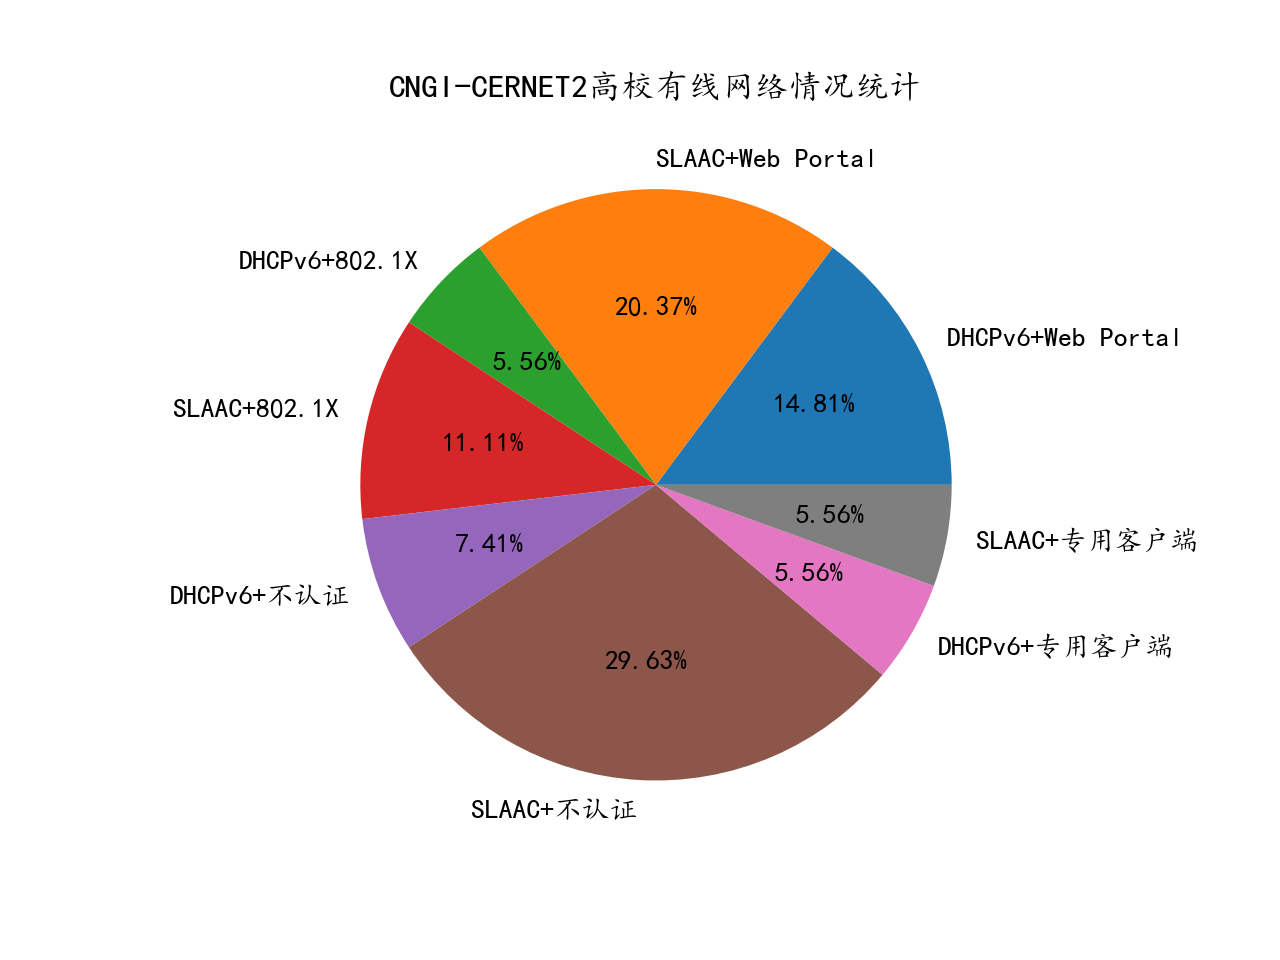
\includegraphics[width=0.49\textwidth]{figures/CNGI_CERNET2_wired.png}}
    \subcaptionbox{无线网络\label{fig:CNGI_CERNET2_wireless}}
    {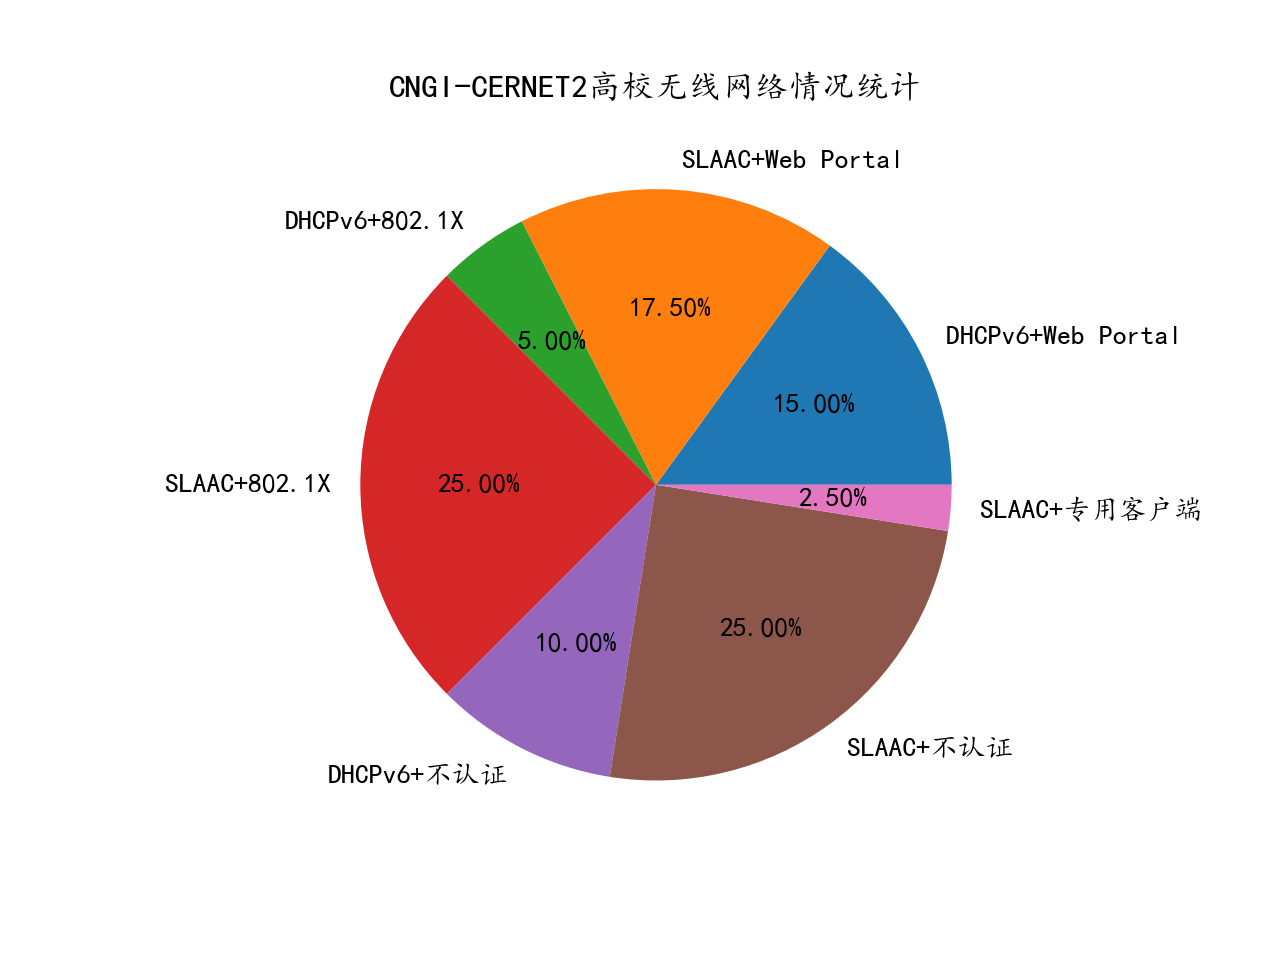
\includegraphics[width=0.49\textwidth]{figures/CNGI_CERNET2_wireless.png}}
    \caption{CNGI-CERNET2高校网络情况统计}
    \label{fig:CNGI_CERNET2_statistic}
  \end{figure}
  
  所有高校的无线网络全部采用基于无线控制器的架构,即各AP不能对自身进行配置和管理,仅仅作为WLAN系统中的一部分,而由AC对所有AP进行统一集中管理的组网模式。在基于无线控制器的无线网络架构下,尽管802.11以及用户认证相关的管理帧均由AP转发至AC处理,但用户发送的数据帧仍有集中转发与本地转发的两种模式。
  
  在用户认证手段方面,主要有802.1X认证、Web Portal认证以及不认证这三类方式,采用PPPoE以及其他定制客户端的认证手段较少。其中802.1X认证手段在无线网络中占比达30\%,远高于有线网络中的16.67\%,这是由于在无线网络中存在用户漫游的需求,802.1X认证方式能够在用户漫游时避免反复认证从而带来更友好的用户体验,而Web Portal认证方式由于其对设备连接性的支持较差,因此在无线网络中被采纳的比重有所下降。同时,对IPv6地址尚未进行用户认证管理的高校也占据了很高的比例,在有线网络与无线网络中分别为37.04\%与35\%。在各高校尚未对IPv6地址进行定制化管控时,向其推广部署用户身份识别与溯源系统面临的阻力将较小,更有利于向网络管理员建议采纳适宜用户身份识别与溯源的认证方式,因此本文将分析各类系统设计方案的优缺点,以选择最为合适的方案推动各高校部署。
  
  在地址配置方式上,DHCPv6与SLAAC两种方式在有线网络与无线网络中均有较大占比。在用户接入设备方面,无线设备主要是手机与笔记本,其中Android手机与iOS手机几乎占据了全部的手机份额,笔记本也以Windows系统与MacOS系统为主,通过有线接入的设备主要有个人电脑与静态配置地址的服务器,以及门禁、刷卡机等嵌入式设备。
  
  本文将各种常见的网络场景总结如图\ref{fig:NIDTGA_network_scenarios},其中忽略了对用户个人设备不进行认证这一类情况以推动各高校对IPv6地址实施管控,更好地支持用户身份识别与溯源系统的应用。可见,当面临实际应用落地时,用户身份识别与溯源系统需要支持大量的网络场景,每一种场景都要求用户身份识别与溯源系统进行定制的设计与实现。本文将以地址配置方式为一级分类,针对校园网络可能采取的认证手段设计与测试用户身份识别与溯源系统,并给出推广时的部署方案。

  \begin{figure}[ht]
    \centering
    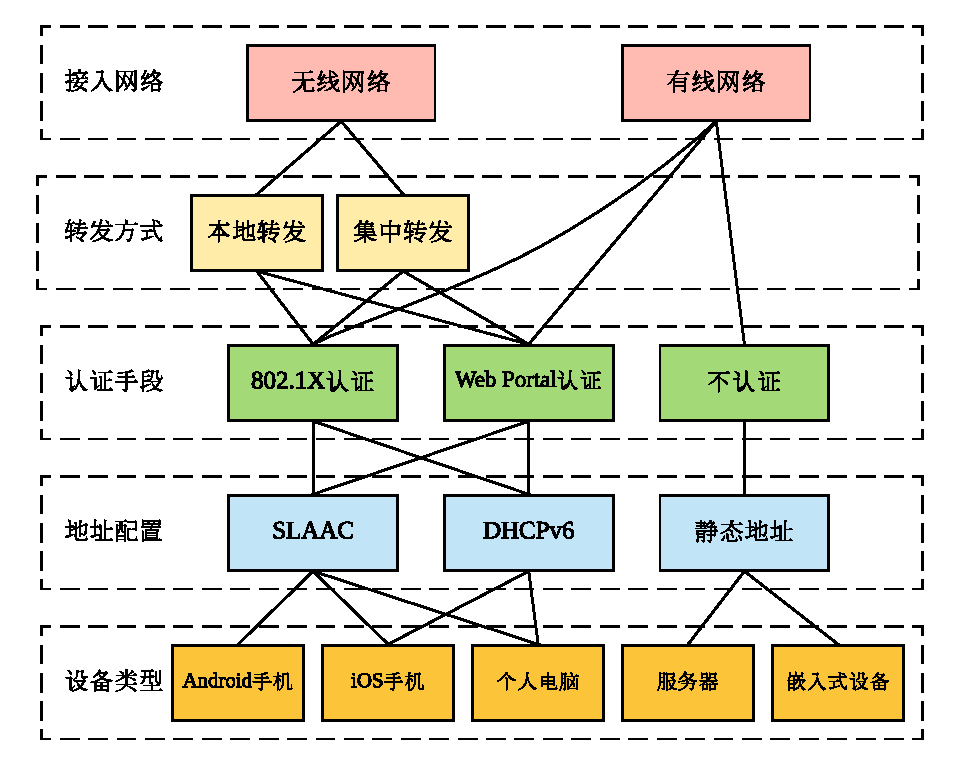
\includegraphics[width=0.9\textwidth]{NIDTGA_network_scenarios.pdf}
    \caption{用户身份识别与溯源系统需要支持的网络场景汇总}
    \label{fig:NIDTGA_network_scenarios}
  \end{figure}


  \section{DHCPv6下的用户身份识别与溯源系统}
  \label{NIDTGA:DHCPv6}
  由于DHCPv6采用集中式的有状态地址管理,用户接入时获得的IPv6地址由DHCPv6服务器决定,因此在DHCPv6配置地址的网络环境下适合采纳NIDTGA地址生成方案,并且一般不需要将其生成方案实现在用户设备端,有利于用户身份识别与溯源系统以用户无感知的方式推广部署。但是,由于NIDTGA生成地址时向IPv6接口标识中嵌入用户身份,因此用户接入网络时必须有身份认证这一过程,网络中不同的认证手段将影响到用户身份识别与溯源系统中认证系统与地址生成系统的交互逻辑。
  本节将首先给出用户身份识别与溯源系统在DHCPv6地址配置下的整体架构设计,然后对扩展DHCPv6认证、Web Portal认证与二层准入认证这三类认证方式下的设计方案分别展开探讨,并介绍各种方案的实现与部署应用情况,对三种方案进行对比和讨论,最后以校园网为例讨论基于二层准入认证的用户身份识别与溯源系统如何在无线网络与有线网络中进行部署推广。

    \subsection{用户身份识别与溯源系统整体架构}
    \label{NIDTGA:DHCPv6:architecture}
    本文设计的用户身份识别与溯源系统整体架构如图\ref{fig:DHCPv6_system_architecture}所示。系统中主要包含:
    \begin{enumerate}[1{)}]
      \item \textbf{认证控制设备}:网络中对用户接入进行认证控制的网络设备,一般为AC、接入交换机或宽带接入服务器等。用户所有流量均通过认证控制设备后才能进行跨子网的转发,认证控制设备将根据用户设备的认证情况,决定用户流量的转发策略。
      \item \textbf{认证管理服务器}:保存用户认证数据库信息的服务器。根据网络中认证手段的不同,具体形式将发生变化,在扩展DHCPv6认证时为一台记录了用户名与密码等匹配信息数据库的认证管理服务器;在采用Web Portal认证时,认证管理服务器将包含提供认证页面的Web Portal服务器与提供实际认证能力的AAA服务器;在二层准入认证时为AAA服务器。
      \item \textbf{密钥管理服务器}:向组织管理员提供NIDTGA地址生成密钥更新服务的网页服务器。组织管理员通过访问该密钥更新服务提交新密钥的更新请求,其负责将新密钥与生效时间发送给DHCPv6服务器与追溯服务器。
      \item \textbf{DHCPv6服务器}:采用NIDTGA地址生成方式为用户设备配置IPv6地址的服务器。在生成地址前需要与组织内的认证管理服务器同步可以用于标识用户的信息,比如用户设备MAC地址。
      \item \textbf{追溯服务器}:提供用户身份溯源服务的服务器。在单个组织内部署时,组织可自行部署一台追溯服务器以保存组织DHCPv6服务器上传的密钥更新历史。在用户身份识别与溯源系统在多个组织进行部署推广后,应部署一台全局唯一的追溯服务器,由具有用户身份溯源权限的审计方进行控制,用于保存各个组织的密钥更新历史,提供根据IPv6地址查询用户身份的服务。
    \end{enumerate}

    \begin{figure}[ht]
      \centering
      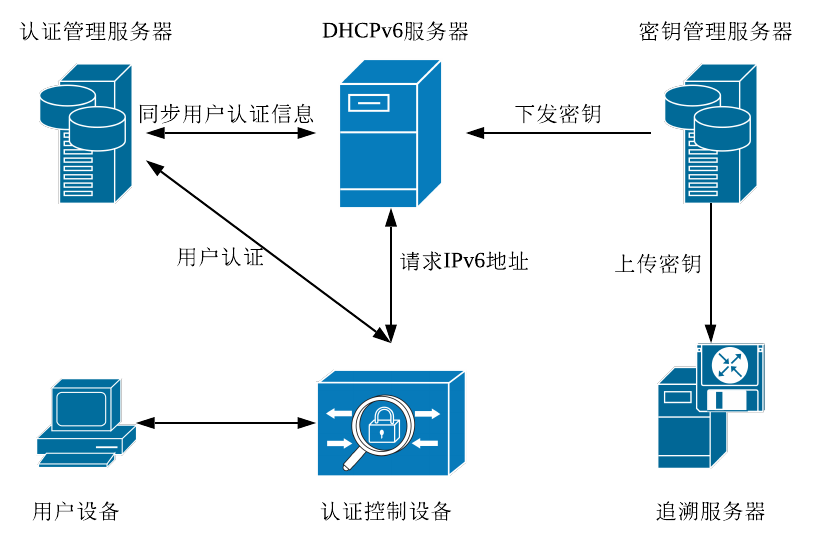
\includegraphics[width=0.7\textwidth]{DHCPv6_system_architecture.png}
      \caption{DHCPv6下用户身份识别与溯源系统整体架构}
      \label{fig:DHCPv6_system_architecture}
    \end{figure}

    在用户通过用户身份识别与溯源系统接入网络时,其数据流量将被认证控制设备阻截,必须首先完成用户身份的认证。认证管理服务器在用户通过认证后将标识认证用户的相关信息同步给DHCPv6服务器。在用户设备请求配置地址时,DHCPv6服务器将根据MAC地址等与用户设备相关联的标识,将请求地址配置的设备与已经完成认证的设备进行匹配,以确认用户身份并为其生成和配置NIDTGA地址。

    根据具体认证手段的不同,用户认证流程与认证管理服务器的形式都将发生变化,在认证管理服务器与DHCPv6服务器之间用于标识同一用户设备的信息也将发生变动,DHCPv6服务器内部生成与配置IPv6地址的逻辑也需要进行相应的更改。下面,本文针对三种不同的认证手段展开讨论,研究在不同的认证流程下用户身份识别与溯源系统的设计方案。

    \subsection{基于扩展DHCPv6协议认证的系统设计}
    \label{NIDTGA:DHCPv6:client}
    在网络中没有采用其他认证手段的情况下,仅通过DHCPv6协议完成用户身份的认证,必须扩展DHCPv6报文的语义,将用户的认证信息添加到DHCPv6报文中。尽管DHCPv6协议标准中没有定义用于携带用户身份信息的选项,但DHCPv6报文的结构使我们可以很容易地向其中添加自定义选项以支持用户认证。本文自定义DHCPv6选项如表\ref{tab:custom_dhcpv6_options}所示。
    \begin{table}[htb]
      \centering
      \begin{minipage}[t]{\linewidth}
        \caption{DHCPv6自定义选项表}
        \label{tab:custom_dhcpv6_options}
        \begin{tabularx}{\linewidth}{cc>{\centering\arraybackslash}X}
          \toprule[1.5pt]
          {\heiti 名称} & {\heiti 编号} & {\heiti 描述} \\\midrule[1pt]
          用户身份标识NID & 101 & 用于在Solicit报文与Request报文中携带用户NID \\ 
          随机数nonce & 102 & 用于在Advertise报文中携带用于密码哈希的随机数 \\ 
          密码MD5哈希 & 103 & 用于在Request报文中携带用户密码结合随机数使用MD5摘要算法哈希后的值 \\ 
          \bottomrule[1.5pt]
        \end{tabularx}
      \end{minipage}
    \end{table}

    同时,为了指示用户NID错误、密码错误等情况,本文利用DHCPv6标准的OPTION\_STATUS\_CODE选项(Option 13),对其携带的状态码进行扩展,可在DHCPv6服务器回复设备的Advertise报文或Reply报文中使用。自定义状态码如表\ref{tab:custom_dhcpv6_status_code}所示。
    \begin{table}[htb]
      \centering
      \begin{minipage}[t]{\linewidth} 
        \caption{DHCPv6自定义状态码表}
        \label{tab:custom_dhcpv6_status_code}
        \begin{tabularx}{\linewidth}{cc>{\centering\arraybackslash}X}
          \toprule[1.5pt]
          {\heiti 名称} & {\heiti 值} & {\heiti 描述} \\\midrule[1pt]
          NID错误 & 129 & 用于NID格式错误或NID在用户数据库中不存在等场景 \\ 
          密码错误 & 130 & 用于密码MD5值与用户数据库中密码的MD5值不匹配的场景 \\ 
          其他错误 & 131 & 用于DHCPv6服务器暂时无法分配IPv6地址的情况 \\
          \bottomrule[1.5pt]
        \end{tabularx}
      \end{minipage}
    \end{table}

    在未启用其他认证手段的DHCPv6配置地址网络中,当用户设备接入时,设备将收到网关公告的Managed位置位的RA报文,设备操作系统将使用内核协议栈中的DHCPv6客户端模块发起IPv6地址配置请求。但操作系统内核的协议栈是不支持自定义的DHCPv6选项的,因此用户身份识别与溯源系统必须在用户设备中禁用内核的DHCPv6客户端,采用定制的DHCPv6客户端输入用户NID与密码进行登录。

    DHCPv6服务器处需要维护用户地址预分配表与用户地址分配表,结构如表\ref{tab:custom_dhcpv6_preallocated}与表\ref{tab:custom_dhcpv6_allocated}所示。

    \begin{table}[htb]
      \centering
      \begin{minipage}[t]{\linewidth} 
        \caption{用户地址预分配表}
        \label{tab:custom_dhcpv6_preallocated}
        \begin{tabularx}{\linewidth}{>{\centering\arraybackslash}Xc>{\centering\arraybackslash}Xcc}
          \toprule[1.5pt]
          {\heiti 设备DUID} & {\heiti 用户NID} & {\heiti NIDTGA地址} & {\heiti 随机数nonce} & {\heiti 过期时间} \\\midrule[1pt]
          000100012537f6 19141877532dbe & 80002888b1 & 2402:f000:6:1c01: 6c28:70f1:be03:efe6 & 121 & 1583754484 \\ 
          \multicolumn{5}{c}{...} \\
          \bottomrule[1.5pt]
        \end{tabularx}
      \end{minipage}
    \end{table}

    \begin{table}[htb]
      \centering
      \begin{minipage}[t]{\linewidth} 
        \caption{用户地址分配表}
        \label{tab:custom_dhcpv6_allocated}
        \begin{tabularx}{\linewidth}{>{\centering\arraybackslash}Xc>{\centering\arraybackslash}Xc}
          \toprule[1.5pt]
          {\heiti 设备DUID} & {\heiti 用户NID} & {\heiti NIDTGA地址} & {\heiti 过期时间} \\\midrule[1pt]
          000100012537f6 19141877532dbe & 80002888b1 & 2402:f000:6:1c01: 6c28:70f1:be03:efe6 & 1583755084\\
          \multicolumn{4}{c}{...} \\
          \bottomrule[1.5pt]
        \end{tabularx}
      \end{minipage}
    \end{table}

    用户的认证流程如图\ref{fig:DHCPv6_custom_client}所示:
    \begin{enumerate}[1{)}]
      \item 用户在定制的DHCPv6客户端中输入NID与密码,点击登录。
      \item 定制DHCPv6客户端构建Solicit报文,添加NID作为Option 101,向链路中进行广播。
      \item DHCPv6服务器收到Solicit报文后,提取NID,将NID与当前时间拼接后使用IDEA密钥对其进行加密,生成NIDTGA地址。
      \item DHCPv6服务器构建Advertise报文,其中提供NIDTGA地址的配置,同时生成一个随机数作为Option 102添加到Advertise报文中,回复该设备,同时将该设备DUID、NID、NIDTGA地址、随机数nonce等关系插入表\ref{tab:custom_dhcpv6_preallocated}。
      \item 定制DHCPv6客户端提取Advertise报文中Option 102携带的随机数nonce,与用户密码拼接后,使用MD5信息摘要算法对其进行哈希,将NID作为Option 101、密码哈希值作为Option 103添加到Request报文中进行回复。
      \item DHCPv6服务器提取Request报文中携带的DUID、NID、密码MD5哈希值,根据DUID与NID查询表\ref{tab:custom_dhcpv6_preallocated}比较判断一致性,并获取对应的nonce。
      \item DHCPv6服务器将NID与nonce发送给认证管理服务器,获取对应用户密码与nonce值哈希后的密文,与用户Request报文中Option 103携带的值进行比较。
      \item 若用户认证成功,则构造Reply报文提供NIDTGA地址的配置信息,分配表\ref{tab:custom_dhcpv6_preallocated}中的NIDTGA地址,将对应表项从表\ref{tab:custom_dhcpv6_preallocated}中删除,并插入表\ref{tab:custom_dhcpv6_allocated}中;若用户登录失败,则构造Reply报文,携带指示失败的错误码回复用户设备,并删除表\ref{tab:custom_dhcpv6_preallocated}中的对应表项。
      \item 客户端根据Reply报文中提供的IPv6地址与租约时间等信息,配置用户设备的网络适配器,接入网络。
    \end{enumerate}

    \begin{figure}[ht]
      \centering
      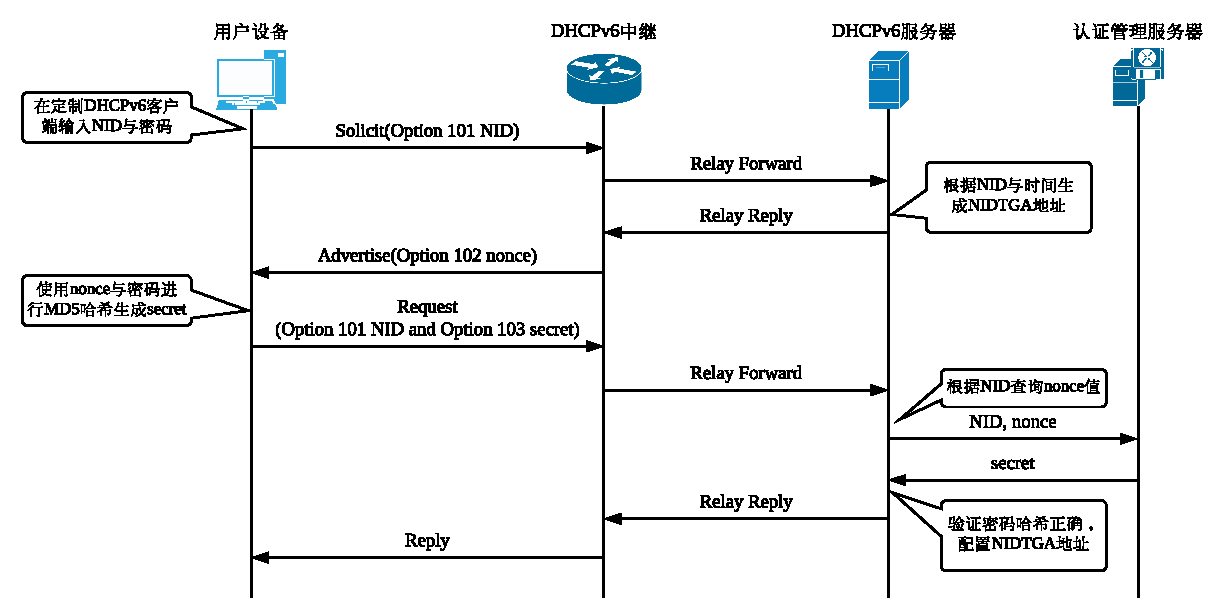
\includegraphics[width=\textwidth]{DHCPv6_custom_client.pdf}
      \caption{DHCPv6下扩展DHCPv6协议认证的用户身份识别与溯源系统时序}
      \label{fig:DHCPv6_custom_client}
    \end{figure}

    \subsection{基于Web Portal认证的系统设计}
    \label{NIDTGA:DHCPv6:portal}
    在大多数的网络环境中,为了限制网络资源的使用、对网络用户进行管理,网络管理者均会借助专用的认证手段对网络接入进行认证控制,其中Web Portal认证由于其轻量级和对用户的友好性得到了广泛的应用。在一般的Web Portal认证场景下,用户设备接入网络后,将根据标准的DHCPv6四步交互获得IPv6地址,认证控制设备将监听DHCPv6报文交互过程,与Web Portal认证系统进行交互,请求并记录包含设备所配置的IPv6地址、设备MAC地址等信息的绑定表项,表项中包含用户流量转发规则;当用户使用该IPv6地址访问网络时,若用户未认证、IPv6地址对应表项转发规则为重定向至认证系统,则认证控制设备将引导用户重定向至Web Portal认证网站;在用户认证通过后,Web Portal认证系统将下发该IPv6地址的新的流量转发规则给认证控制设备,允许该用户IPv6地址的流量访问网络。

    但是,NIDTGA地址生成逻辑与Web Portal认证的地址配置流程是冲突的:用户身份识别与溯源系统需要先获取用户身份后生成NIDTGA地址配置用户设备,而Web Portal认证则先配置设备IPv6地址后进行用户身份认证。没有获取IPv6地址则用户无法访问Web Portal进行认证,而不完成认证,用户身份识别与溯源系统又无法为用户设备生成NIDTGA地址并进行配置,用户认证与地址分配这两个过程在Web Portal认证手段下形成了一种死锁的关系。

    为了调和上述矛盾,我们需要采纳一种地址二次分配的过程:
    \begin{enumerate}[1{)}]
      \item 首先给用户设备分配一个用于访问Web Portal网站进行认证的临时IPv6地址,并指示认证控制设备对这类临时地址的流量始终进行重定向到Web Portal网站的操作;
      \item 在用户通过认证后,生成NIDTGA地址并对用户设备IPv6地址进行重新配置,并下发新的流量控制规则给认证控制设备。
    \end{enumerate}

    尽管DHCPv6标准\cite{RFC8415}中定义了由DHCPv6服务器对接入设备IPv6地址进行地址重配置的Reconfigure报文,但经过测试,目前通用设备的操作系统内核中的DHCPv6客户端均不支持对Reconfigure报文的处理,因此难以在DHCPv6服务器端主动发起地址重新配置的过程。在设备端,除去设备网络适配器重新连接网络的情况,重新配置地址的过程只在当前持有的IPv6地址续约时间来临时发起,因此必须将设备的临时IPv6地址租约时间设置得非常短,以确保用户在认证通过后迅速发起续约过程并重新配置地址。

    在这种情况下,DHCPv6服务器需要维护用户设备获取临时IPv6地址的状态与用户设备持有NIDTGA地址的状态,分别如表\ref{tab:web_portal_temporary}与表\ref{tab:web_portal_nidtga}所示。

    \begin{table}[htb]
      \centering
      \begin{minipage}[t]{\linewidth} 
        \caption{临时地址状态表}
        \label{tab:web_portal_temporary}
        \begin{tabularx}{\linewidth}{>{\centering\arraybackslash}Xccc}
          \toprule[1.5pt]
          {\heiti 设备DUID} & {\heiti 临时IPv6地址} & {\heiti 过期时间} & {\heiti 续约次数} \\\midrule[1pt]
          000100012537f619141877532dbe & 2402:f000:6:1c01::1 & 1583754484 & 3 \\ 
          \multicolumn{4}{c}{...} \\
          \bottomrule[1.5pt]
        \end{tabularx}
      \end{minipage}
    \end{table}

    \begin{table}[htb]
      \centering
      \begin{minipage}[t]{\linewidth} 
        \caption{NIDTGA地址状态表}
        \label{tab:web_portal_nidtga}
        \begin{tabularx}{\linewidth}{>{\centering\arraybackslash}Xc>{\centering\arraybackslash}Xc}
          \toprule[1.5pt]
          {\heiti 设备DUID} & {\heiti 用户NID} & {\heiti NIDTGA地址} & {\heiti 过期时间} \\\midrule[1pt]
          000100012537f6 19141877532dbe & 80002888b1 & 2402:f000:6:1c01: 6c28:70f1:be03:efe6 & 1583754484 \\ 
          00030001548998 923171 & 80002888b2 & 2402:f000:6:1c01: 12b7:1321:f025:1642 & 1583754943 \\ 
          \multicolumn{4}{c}{...} \\
          \bottomrule[1.5pt]
        \end{tabularx}
      \end{minipage}
    \end{table}


    本文设计Web Portal认证下的用户身份识别与溯源方案用户接入流程如图\ref{fig:DHCPv6_web_portal}所示:
    \begin{enumerate}[1{)}]
      \item 用户设备接入网络,通过标准的DHCPv6协议获取临时IPv6地址。
      \item DHCPv6服务器在收到用户设备的地址配置请求报文后,先根据设备DUID查询表\ref{tab:web_portal_nidtga},若不存在则从临时IPv6地址池中选择临时IPv6地址进行分配,租约时间设置为$T1=3s$,$T2=5s$,即3秒发送Renew报文,5秒发送Rebind报文,并将用户DUID、临时IPv6地址等关系插入表\ref{tab:web_portal_temporary};否则将根据表\ref{tab:web_portal_nidtga}中对应表项为其分配NIDTGA地址。
      \item 在用户设备请求临时IPv6地址过程中,认证控制设备将与Web Portal认证系统交互,获取用户临时IPv6地址绑定表项,规则为将用户流量重定向至Web Portal网站。
      \item 用户认证前,用户设备可能在临时IPv6地址租约到期之际多次向DHCPv6服务器发送Renew报文进行续约,以确保用户能够访问Web Portal网站,DHCPv6服务器将更新表\ref{tab:web_portal_temporary}中相应的过期时间与续约次数,并根据续约次数调整临时IPv6地址的租约时间。
      \item 用户使用临时IPv6地址通过浏览器访问网络时,将被重定向至Web Portal网站。
      \item 用户提交NID与密码完成认证,通过后,Web Portal认证系统将认证用户的NID、临时IPv6地址发送给DHCPv6服务器。
      \item DHCPv6服务器向表\ref{tab:web_portal_temporary}中查询临时IPv6地址对应认证用户设备的DUID,并根据用户NID与时间生成NIDTGA地址,将DUID、NID、NIDTGA地址等信息插入表\ref{tab:web_portal_nidtga}中。
      \item 用户设备再次发起对临时IPv6地址的续约流程,DHCPv6服务器根据DUID查询表\ref{tab:web_portal_nidtga},若表中存在该DUID,说明用户已认证,则对其续约请求回复立即过期的租约时长,使其发起新的地址配置请求;当设备为NIDTGA地址续约时,DHCPv6服务器检查地址是否与表\ref{tab:web_portal_nidtga}中匹配,若是则回复为其正常续约的Reply报文。
      \item 用户设备续约临时IPv6地址获得的新租约时长为0后,立即通过标准的DHCPv6协议发起新的地址配置请求,DHCPv6服务器根据其DUID查询表\ref{tab:web_portal_nidtga},确认后为其配置NIDTGA地址,并更新表\ref{tab:web_portal_nidtga}中过期时间。
      \item 当认证控制设备一段时间内未检测到用户设备的数据流量时,其向Web Portal认证管理服务器发送用户下线请求,包含用户NIDTGA地址,Web Portal认证管理服务器将对应用户下线,并将NIDTGA地址发送给DHCPv6服务器通知其将用户信息从表\ref{tab:web_portal_nidtga}中删除。
    \end{enumerate}
          
    \begin{figure}[ht]
      \centering
      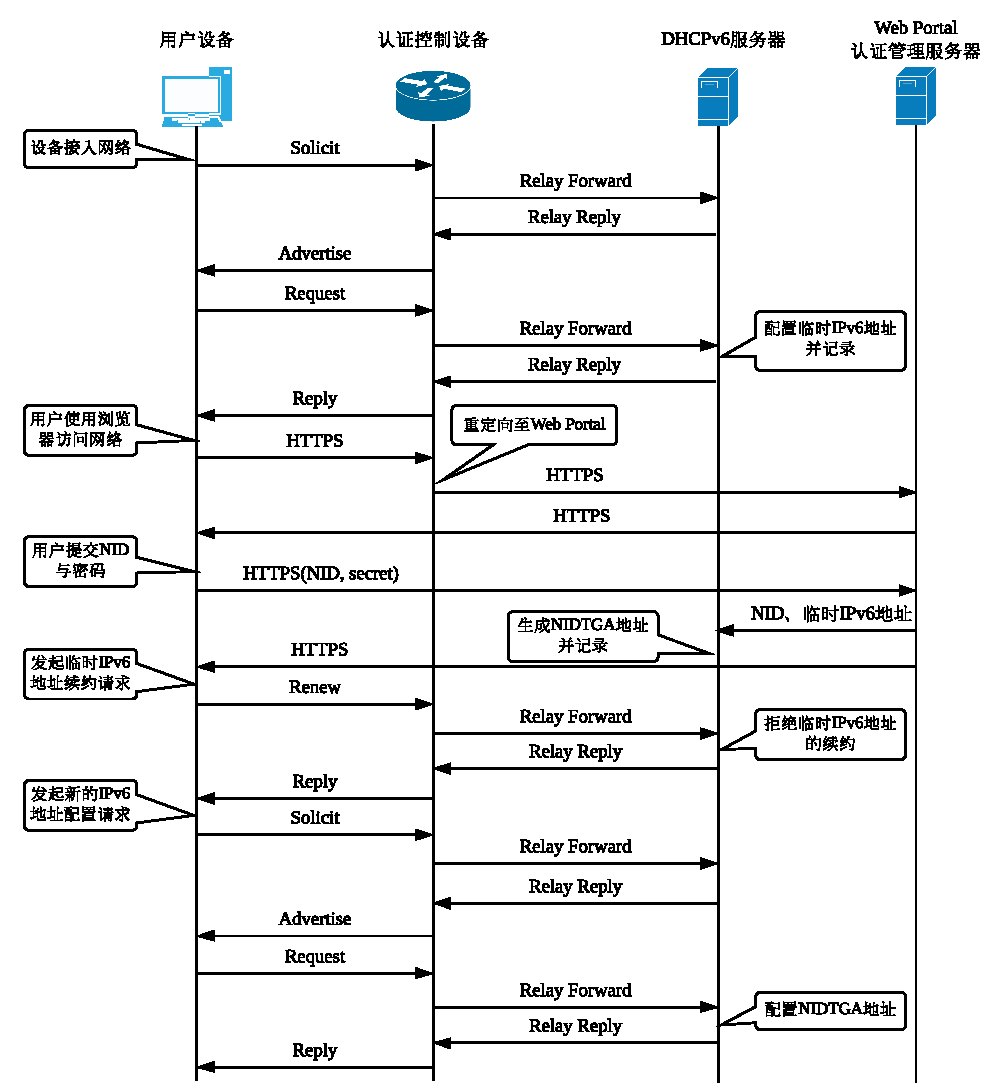
\includegraphics[width=\textwidth]{DHCPv6_web_portal.pdf}
      \caption{DHCPv6下Web Portal认证的用户身份识别与溯源系统时序}
      \label{fig:DHCPv6_web_portal}
    \end{figure}

    值得一提的是,由于临时地址的租约时间短,在未认证之前用户设备将频繁发起续约请求,对网络中的交换机等设备造成较大的负担,因此本文设计了对多次续约的临时地址租约时长进行调整的机制,以减轻网络设备的负担。DHCPv6服务器将在表\ref{tab:web_portal_temporary}中维护每个临时IPv6地址的续约次数,根据用户设备续约次数$n$,采取式\eqref{eq:T1_adjustment}对临时地址的T1时间进行调整,T2与过期时间将分别被设置为T1的$\frac{5}{3}$与$2$倍。
    \begin{equation}
      \label{eq:T1_adjustment}
      T1(n) = \left\{
      \begin{array}{rcl}
        3 & & {n \leq 40} \\
        6 & & {40 < n \leq 70} \\
        30 & & {n > 70}   
      \end{array}
      \right.
    \end{equation}

    本文在此对用户认证成功后配置NIDTGA地址所需的等待时间进行估算。当用户在获得临时地址后2分钟内完成认证,这是用户上网最为常见的情况,用户平均等待1.5秒,至多等待3秒即可获得NIDTGA地址访问网络;当用户在2分钟至5分钟内完成认证,则用户平均等待3秒,至多等待6秒;若用户在5分��内均未完成认证,则我们认为该用户暂时没有认证的意愿,其续约时长为30秒,故用户平均等待15秒,至多等待30秒访问网络。

    对于用户下线后又重新上线的情况,若NIDTGA地址已过期,则情况与用户新上线相同,否则其所需等待的时长与NIDTGA地址的租约时间有关。设DHCPv6服务器将NIDTGA地址的续约时间设置为$T$,用户下线距上一次续约的时长在0到$T$内均匀分布,概率密度为$\frac{1}{T}$。将用户下线后重新上线的行为建模为强度为$\lambda$的泊松过程。设$t$为用户设备IPv6地址最后一次续约至用户下线之间经过的时长,那么在下一次IPv6地址续约来临之前,用户重新认证上线的概率期望可根据式\eqref{eq:reauthenticate_probability}计算。用户重新认证的时间距离用户下线时间的随机变量呈指数分布,因此重新认证后获取新的NIDTGA地址的等待时长期望由式\eqref{eq:reauthenticate_time}计算。若用户平均每5分钟重新认证,即$\lambda = \frac{1}{300}$,NIDTGA地址的续约时间$T=30$秒,则用户在NIDTGA地址过期前重新认证的概率期望为0.048,等待时长期望为14.632秒,可见用户在NIDTGA地址过期前重新认证上线的概率极小,等待时长的期望较短,不会对用户体验造成较大影响。

    \begin{subequations}
      \begin{align}
        E(P(reauthenticate)) &= \int_{0}^{T}{\frac{1}{T}P(N(T - t) \geq 1)dt}=1-\frac{1}{\lambda T}(1 - e^{-\lambda T}) \label{eq:reauthenticate_probability} \\
        E(waiting\_time) &= \int_{0}^{T}{\int_{0}^{T-t_{1}}{(T-t_{1}-t_{2})\lambda e^{-\lambda t_{2}}dt_{2}}dt_{1}} = \frac{T^2}{2}+\frac{1}{\lambda^{2}}(1-e^{-\lambda T})-\frac{T}{\lambda} \label{eq:reauthenticate_time}
      \end{align}
    \end{subequations}

    \subsection{基于二层准入认证的系统设计}
    \label{NIDTGA:DHCPv6:8021X}
    除了Web Portal认证方式外,二层准入认证也是网络接入时常用的认证技术。与Web Portal这种使用三层及以上协议进行认证的技术相比,二层准入认证逻辑更为简单,其认证信息通过用户设备与接入点设备之间的二层数据帧进行携带,在用户认证完成之前不允许认证报文以外的流量通过接入端口,在用户认证通过后流量才可正常转发。802.1X\cite{ieee802ieee}是一个典型的二层准入认证的网络接入控制标准,本文将以此为认证手段进行二层准入认证的用户身份识别与溯源系统研究。
    
    在使用802.1X进行用户身份认证的网络中,用户设备完成802.1X认证后,其操作系统内核DHCPv6客户端发送的DHCPv6报文才能够通过受控端口到达本地链路或其他可达链路中的DHCPv6服务器,进行标准的DHCPv6地址配置流程。为实现用户身份识别与溯源系统,DHCPv6服务器需要根据用户设备发送的DHCPv6报文确定用户身份。

    在DHCPv6服务器的视角中,区分不同设备的标识是设备DUID,而在用户认证时的AAA服务器的视角中,区分设备的标识是设备MAC地址。为了避免对用户设备DHCPv6客户端的侵入式修改以携带用户NID,本文设计以设备MAC地址作为桥梁,令DHCPv6服务器根据MAC地址判断设备是否已经完成认证。尽管用户设备的DUID往往根据设备MAC地址生成,但DHCPv6标准定义的生成方式有三种,且在设备拥有多网卡的情况下生成DUID的MAC地址可能并非实际接入网络发起DHCPv6请求的网络适配器地址,因此通过DUID提取出的MAC地址并不可靠。本文利用RFC 6939\cite{RFC6939}中定义的Client Link-Layer Address选项,指示链路中第一跳DHCPv6中继将用户设备的MAC地址添加到Relay Forward报文的Option 79中。根据Relay Forward报文中该选项所携带的用户设备MAC地址,DHCPv6服务器向AAA服务器处同步的认证用户列表进行查询获得用户NID。

    DHCPv6服务器需要维护已认证设备表与NIDTGA地址分配表,分别记录已在AAA服务器处完成认证的设备信息与用户设备已配置的NIDTGA地址,如表\ref{tab:authorized_devices}与表\ref{tab:802.1X_nidtga}所示。
    \begin{table}[htb]
      \centering
      \begin{minipage}[t]{\linewidth} 
        \caption{已认证设备表}
        \label{tab:authorized_devices}
        \begin{tabularx}{\linewidth}{>{\centering\arraybackslash}X>{\centering\arraybackslash}X>{\centering\arraybackslash}X}
          \toprule[1.5pt]
          {\heiti 设备MAC} & {\heiti 用户NID} & {\heiti 过期时间} \\\midrule[1pt]
          78:31:c1:c8:10:8c & 80002888b1 & 1583754484 \\ 
          \multicolumn{3}{c}{...} \\
          \bottomrule[1.5pt]
        \end{tabularx}
      \end{minipage}
    \end{table}

    \begin{table}[htb]
      \centering
      \begin{minipage}[t]{\linewidth} 
        \caption{NIDTGA地址分配表}
        \label{tab:802.1X_nidtga}
        \begin{tabularx}{\linewidth}{>{\centering\arraybackslash}Xcc>{\centering\arraybackslash}Xc}
          \toprule[1.5pt]
          {\heiti 设备DUID} & {\heiti 设备MAC地址} & {\heiti 用户NID} & {\heiti NIDTGA地址} & {\heiti 过期时间} \\\midrule[1pt]
          000100012537f6 19141877532dbe & 78:31:c1:c8:10:8c & 80002888b1 & 2402:f000:6:1c01: 6c28:70f1:be03:efe6 & 1583754484 \\ 
          \multicolumn{3}{c}{...} \\
          \bottomrule[1.5pt]
        \end{tabularx}
      \end{minipage}
    \end{table}


    因此,用户身份识别与溯源系统在802.1X认证方式下的时序图如图\ref{fig:DHCPv6_802.1X_client}所示:
    \begin{enumerate}[1{)}]
      \item 用户设备接入网络,通过标准802.1X方式完成用户认证;AAA服务器向DHCPv6服务器同步认证用户的MAC地址、用户身份标识NID等信息,DHCPv6服务器将其插入表\ref{tab:authorized_devices}中;
      \item 用户设备通过标准DHCPv6客户端发送Solicit报文,经过的第一个DHCPv6中继将用户设备MAC地址加入Relay Forward报文;
      \item DHCPv6服务器解析Option 79选项获得MAC地址,查询表\ref{tab:authorized_devices}获取用户NID,并结合当前时间生成NIDTGA地址,将对应表项从表\ref{tab:authorized_devices}中删除,将DUID、MAC、NID、NIDTGA地址等信息生成表项插入表\ref{tab:802.1X_nidtga}中;
      \item DHCPv6服务器根据生成的NIDTGA地址向用户设备回复Advertise报文;
      \item 用户设备发送Request报文正式请求IPv6地址,第一跳DHCPv6中继同样将设备MAC地址加入Relay Forward报文;
      \item DHCPv6服务器在表\ref{tab:802.1X_nidtga}中查询用户设备DUID、MAC、NIDTGA地址等,确认一致后回复Reply报文进行地址配置,并根据租约更新表\ref{tab:802.1X_nidtga}中过期时间。
    \end{enumerate}
    
    \begin{figure}[ht]
      \centering
      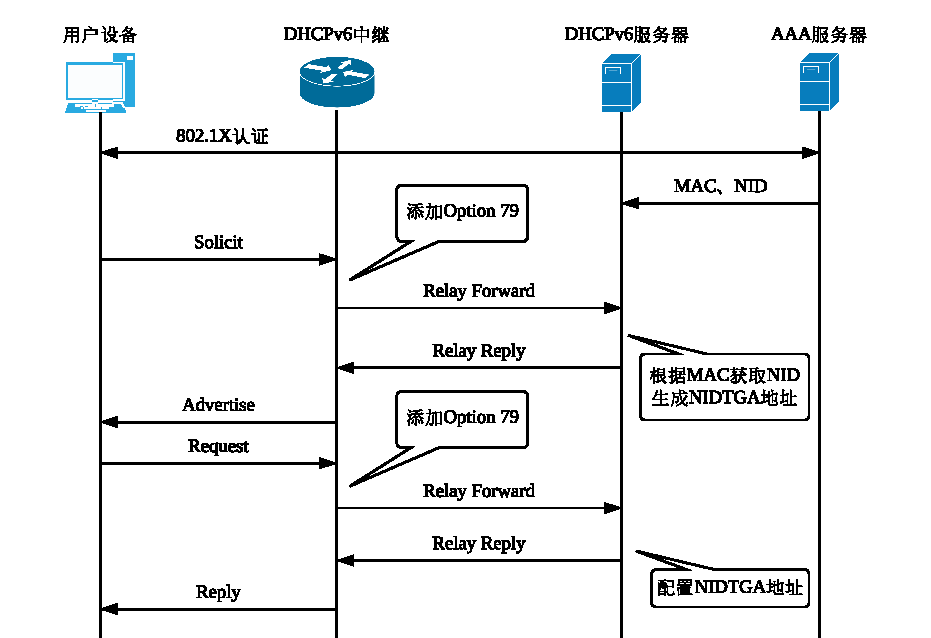
\includegraphics[width=0.9\textwidth]{DHCPv6_8021X_client.pdf}
      \caption{DHCPv6下802.1X认证的用户身份识别与溯源系统时序}
      \label{fig:DHCPv6_802.1X_client}
    \end{figure}


    \subsection{三种系统设计方案的实现部署情况}
    \label{NIDTGA:DHCPv6:implement}

        \subsubsection{基于扩展DHCPv6认证的系统设计方案}
        \label{NIDTGA:DHCPv6:implement:custom}
        目前,基于扩展DHCPv6认证的系统设计方案已经开发完成,在清华大学、北京大学、北京邮电大学、上海交通大学与东南大学五所高校进行了部署,并通过了288项目的验收。系统中主要包含以下几个部分,本文作者开发并重构了其中地址生成系统的代码与Windows客户端的代码,其他部分的代码主要由赛尔网络公司开发完成:
        \begin{enumerate}[1{)}]
          \item \textbf{用户注册系统}:如图\ref{fig:user_register_system}所示,包括用户登录与注册等功能,师生们填写真实信息后完成系统注册,获得用户身份标识NID。
            \begin{figure}[ht]
              \centering
              \subcaptionbox{登录页面\label{fig:user_register_system_0}}
              {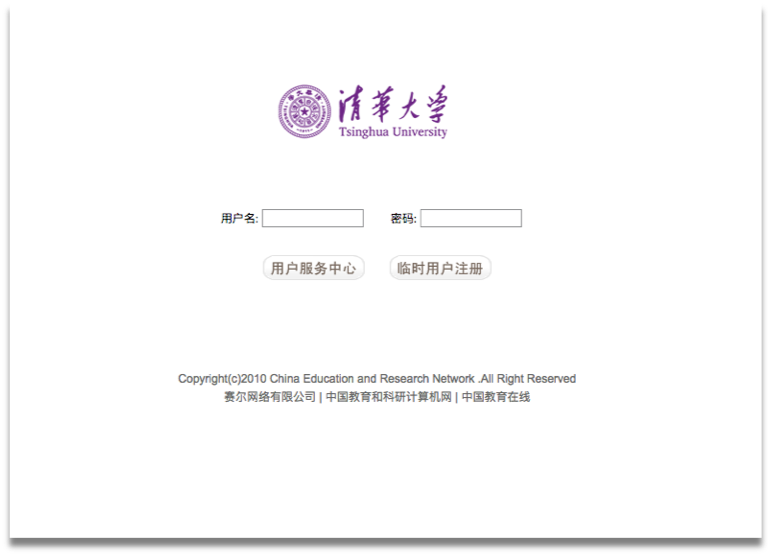
\includegraphics[height=4cm]{user_register_system_0.png}}
              \hspace{2em}
              \subcaptionbox{注册页面\label{fig:user_register_system_1}}
              {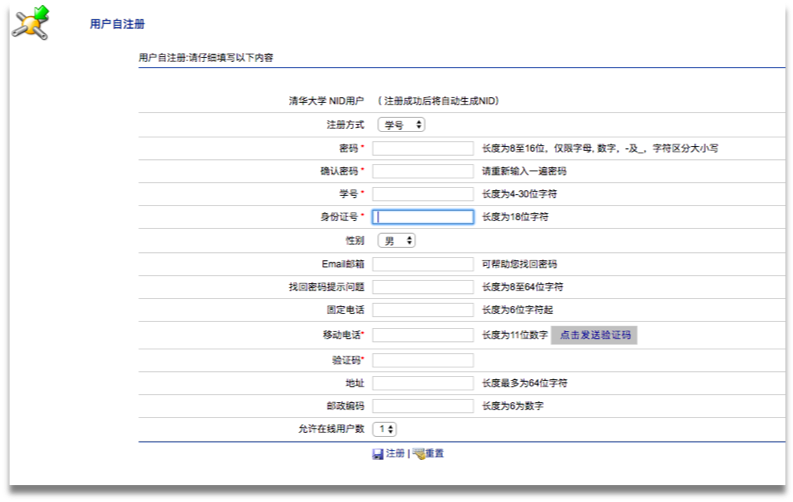
\includegraphics[height=4cm]{user_register_system_1.png}}
              \caption{288项目用户注册系统}
              \label{fig:user_register_system}
            \end{figure}
          \item \textbf{定制DHCPv6客户端}:客户端采用C\#进行实现,需要用户在设备上进行安装,用于连接系统后的认证,其将关闭操作系统内核的DHCPv6模块,启用自身的DHCPv6客户端功能进行IPv6地址请求,并配置设备网卡。Windows7/10、MacOS、Linux与Android系统下的客户端均已实现支持,其界面如图\ref{fig:user_custom_client}所示。
            \begin{figure}[ht]
              \centering
              \subcaptionbox{用户登录界面\label{fig:user_custom_client_0}}
              {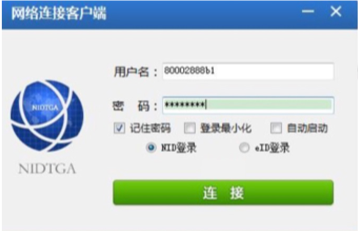
\includegraphics[height=4cm]{user_custom_client_0.png}}
              \hspace{2em}
              \subcaptionbox{认证成功界面\label{fig:user_custom_client_1}}
              {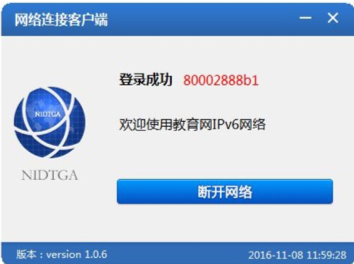
\includegraphics[height=4cm]{user_custom_client_1.png}}
              \caption{288项目用户DHCPv6客户端}
              \label{fig:user_custom_client}
            \end{figure}
          \item \textbf{地址生成系统}:地址生成系统基于ISC DHCP\footnote{ISC DHCP, https://www.isc.org/dhcp/}服务器的开源代码进行开发,主要以其server/dhcpv6.c中void dhcpv6(struct packet *packet)函数为入口,实现了NIDTGA地址的生成方案,修改了其IPv6地址配置的逻辑如图\ref{fig:custom_client_DHCPv6_server_logic}所示,以支持用户认证。
            \begin{figure}[ht]
              \centering
              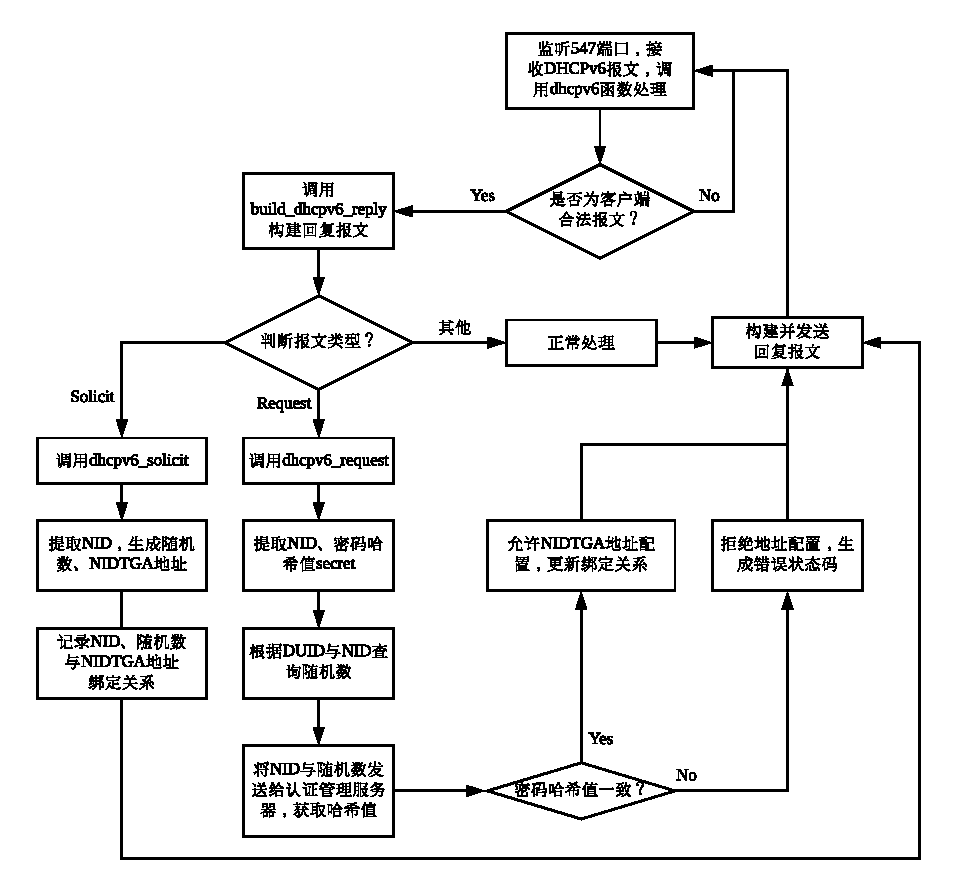
\includegraphics[width=0.9\textwidth]{custom_client_DHCPv6_server_logic.pdf}
              \caption{扩展DHCPv6认证的地址生成系统处理逻辑}
              \label{fig:custom_client_DHCPv6_server_logic}
            \end{figure}
          
          \item \textbf{网络管理系统}:网络管理系统可查看当前网络中的在线用户、SAVI交换机绑定表信息、以及整个系统中的用户注册数量等,如图\ref{fig:DHCPv6_client_deploy_result}所示,五所部署该系统的高校均包含4000以上的注册用户,整个系统的用户数量共计2万人以上。
            \begin{figure}[ht]
              \centering
              \subcaptionbox{清华大学部署情况\label{fig:DHCPv6_client_deploy_Tsinghua}}
              {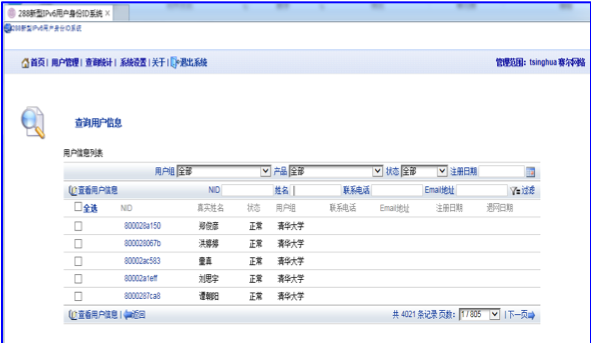
\includegraphics[height=4cm]{DHCPv6_client_deploy_Tsinghua.png}}
              \subcaptionbox{北京大学部署情况\label{fig:DHCPv6_client_deploy_Peking}}
              {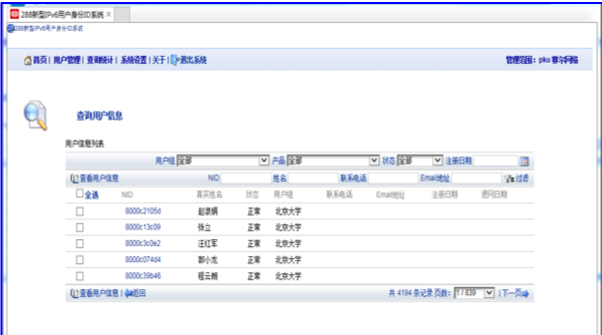
\includegraphics[height=4cm]{DHCPv6_client_deploy_Peking.png}}
              \caption{288项目高校部署情况举例}
              \label{fig:DHCPv6_client_deploy_result}
            \end{figure}
          \item \textbf{身份溯源系统}:身份溯源系统根据IPv6地址溯源用户身份信息,如图\ref{fig:user_trace_system}所示,为保护用户隐私,本文已将用户相关信息从图中抹去。
            \begin{figure}[ht]
              \centering
              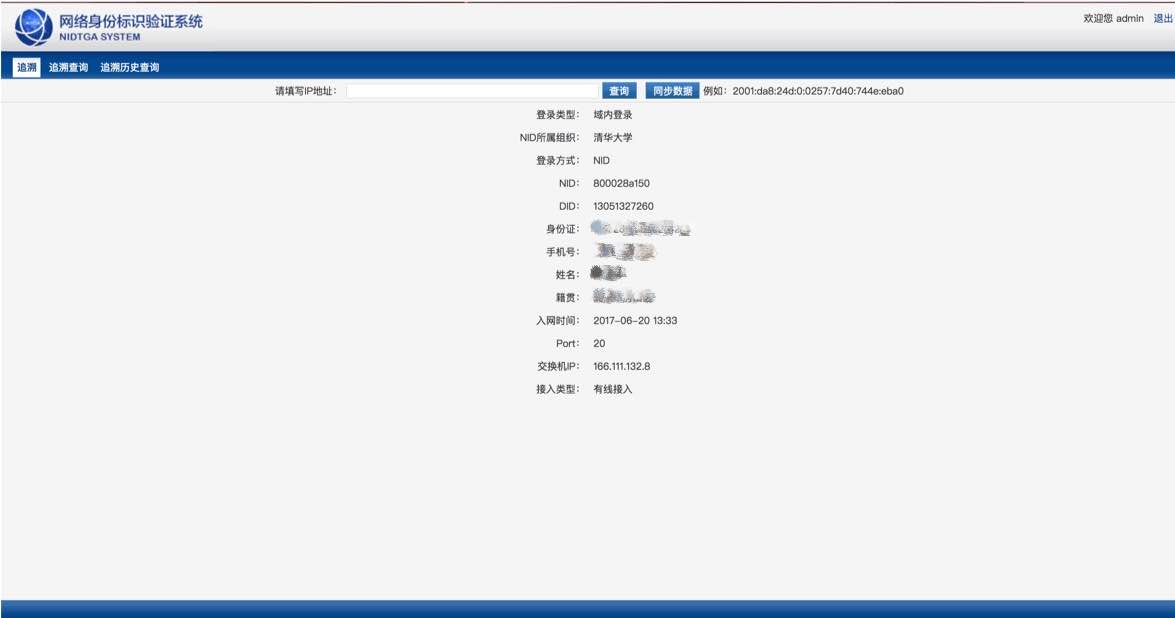
\includegraphics[height=6cm]{user_trace_system.jpeg}
              \caption{288项目身份溯源系统}
              \label{fig:user_trace_system}
            \end{figure}
        \end{enumerate}
    
        \subsubsection{基于Web Portal认证的系统设计方案}
        \label{NIDTGA:DHCPv6:implement:portal}
        基于Web Portal认证的方案已由本文作者独立进行原型系统的实现和验证,系统实现架构如图\ref{fig:DHCPv6_web_portal_implementation}所示。
        \begin{figure}[ht]
          \centering
          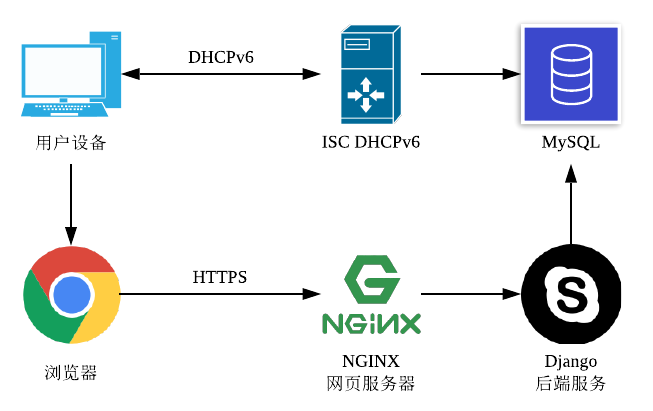
\includegraphics[width=0.6\textwidth]{figures/DHCPv6_web_portal_implementation.png}
          \caption{Web Portal认证的系统实现架构示意}
          \label{fig:DHCPv6_web_portal_implementation}
        \end{figure}
        
        系统主要包含两个部分:
        \begin{enumerate}[1{)}]
            \item \textbf{Web Portal认证系统}:Web Portal认证系统主要为用户提供Web Portal认证的网页服务,并向地址生成系统传递完成认证的用户相关信息。本文采用Django框架\footnote{Django, https://www.djangoproject.com/}开发了Web Portal网站,以MySQL\footnote{MySQL, https://www.mysql.com/cn/}作为用户认证数据库、以Nginx\footnote{Nginx, https://www.nginx.com/}作为网页服务器对其进行了部署测试。其逻辑较为简单,在用户访问时返回认证的HTML页面,在用户提交NID与密码认证后,查询数据库进行比对,返回提示认证成功与否的消息,并将NID、用户IPv6地址、认证时间写入数据库。
            \item \textbf{地址生成系统}:地址生成系统采用基于ISC DHCP服务器的开源代码扩展实现。在DHCPv6服务器配置文件中需要配置两个IPv6地址段,分别作为临时地址与NIDTGA生成地址。代码同样以对其中server/dhcpv6.c中void dhcpv6(struct packet *packet)函数为入口的执行逻辑修改为主,实现了图\ref{fig:web_portal_DHCPv6_server_logic}的过程。
            \begin{figure}[ht]
              \centering
              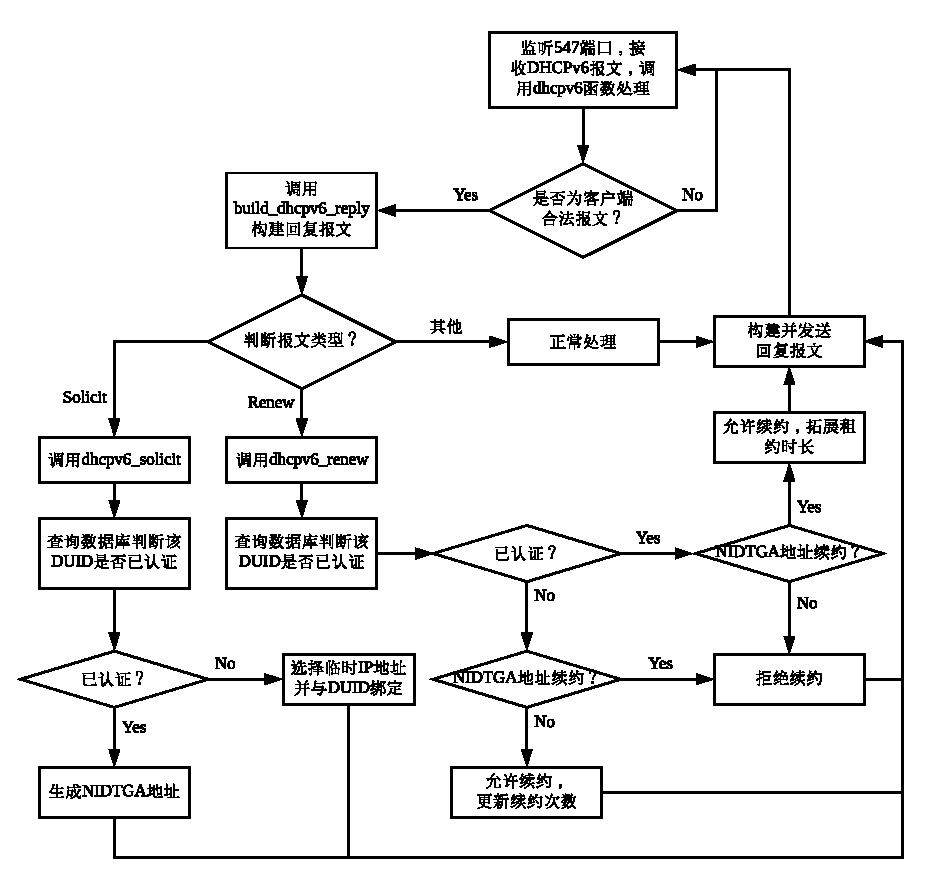
\includegraphics[width=0.9\textwidth]{web_portal_DHCPv6_server_logic.pdf}
              \caption{Web Portal认证的地址生成系统处理逻辑}
              \label{fig:web_portal_DHCPv6_server_logic}
            \end{figure}
        \end{enumerate}
    
        由于其存在较大的性能开销、用户等待延迟等问题,目前未在高校进行推广部署。

        \subsubsection{基于二层准入认证的系统设计方案}
        \label{NIDTGA:DHCPv6:implement:8021X}
        基于二层准入认证方案已由本文作者负责并与清华大学下一代互联网国家重点实验室的工程师合作实现,其实现架构如图\ref{fig:DHCPv6_8021X_implementation}所示。
        
        \begin{figure}[ht]
          \centering
          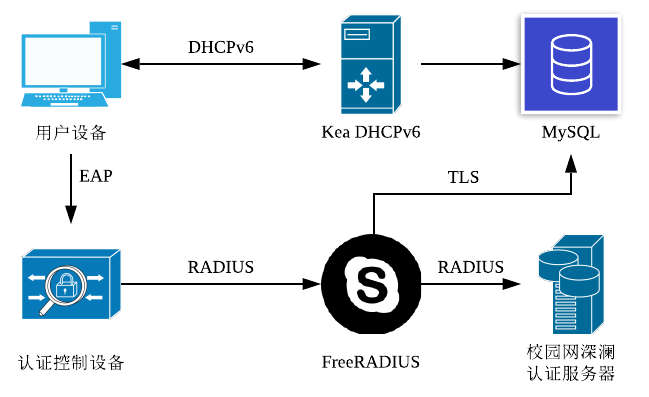
\includegraphics[width=0.6\textwidth]{figures/DHCPv6_8021X_implementation.png}
          \caption{二层准入认证的系统实现架构示意}
          \label{fig:DHCPv6_8021X_implementation}
        \end{figure}
        
        系统主要包含以下两个部分:
        \begin{enumerate}[1{)}]
          \item \textbf{地址生成系统}:基于Kea DHCP\footnote{Kea DHCP, https://www.isc.org/kea/}服务器的开源代码实现,主要包含Hook客户端与独立开发的地址生成服务。Kea DHCPv6服务器在处理用户地址配置请求报文时,使用扩展的Hook作为客户端与地址生成服务进行通信,获取NIDTGA地址,两者关系如图\ref{fig:user_address_generation_system}所示。DHCPv6服务器处的处理逻辑基本保持不变,将选择IPv6地址的过程更改为通过Hook向地址生成服务请求地址。地址生成服务监听传输层7839端口,与Hook建立socket通信,接收MAC地址,查询设备认证信息获得该设备的用户NID,为其生成NIDTGA地址并回复DHCPv6服务器。
            \begin{figure}[ht]
              \centering
              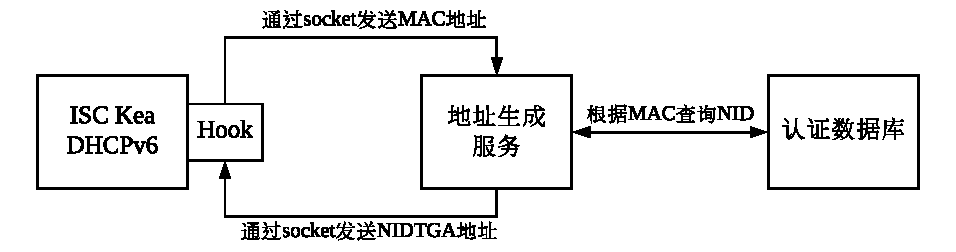
\includegraphics[width=0.9\textwidth]{user_address_generation_system.pdf}
              \caption{二层准入认证的地址生成系统构成示意}
              \label{fig:user_address_generation_system}
            \end{figure}
          \item \textbf{用户认证系统}:基于FreeRADIUS服务器的开源代码实现。为了增强系统部署推广能力,避免用户注册,支持校园网用户使用校园网账号认证,实现用户无感知接入,用户认证系统自动根据用户的校园网账号为其生成用户身份标识NID,并与校园网认证系统进行对接,自身作为RADIUS代理将用户认证请求通过RADIUS报文转发给校园网认证系统,在本地不存储用户密码相关的信息,以实现更好的安全性。
        \end{enumerate}
    
        \begin{figure}[ht]
          \centering
          \subcaptionbox{802.1X认证页面}
          {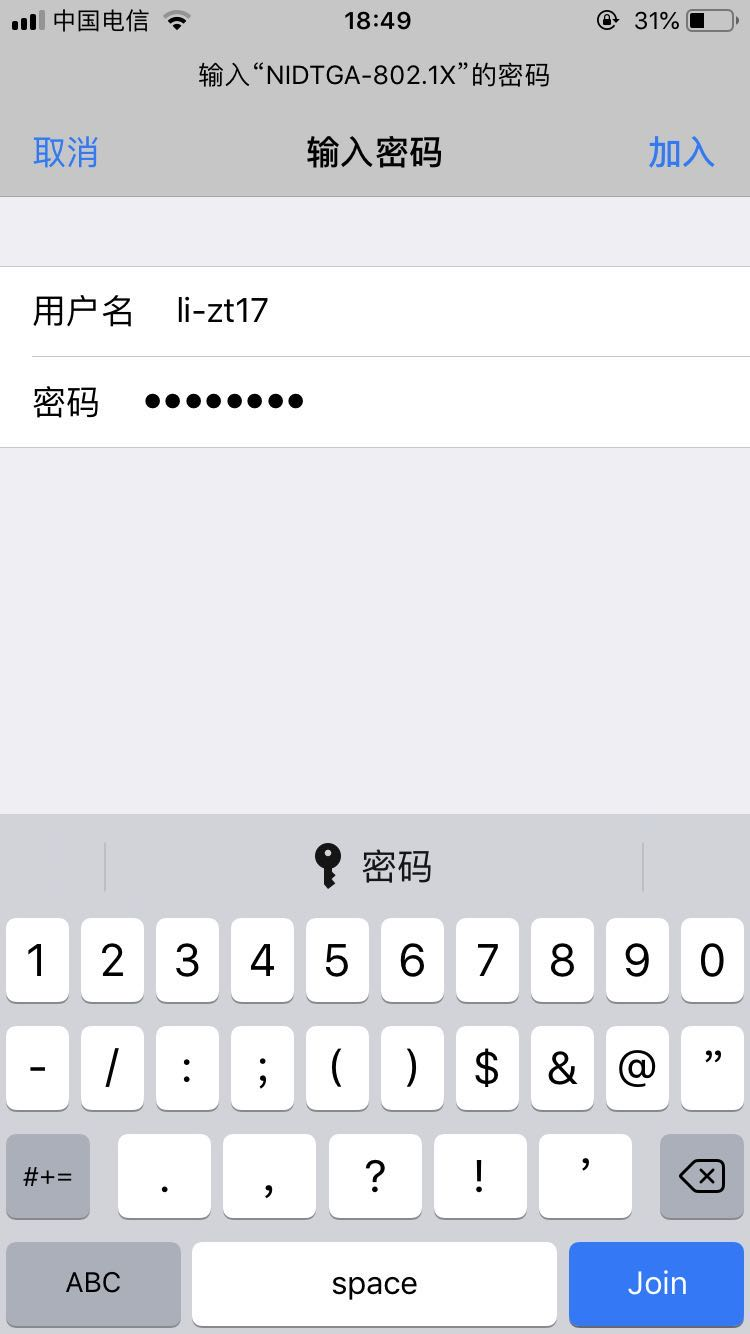
\includegraphics[height=6cm]{DHCPv6_8021X_deploy_0.jpeg}}
          \hspace{2em}
          \subcaptionbox{WiFi连接页面}
          {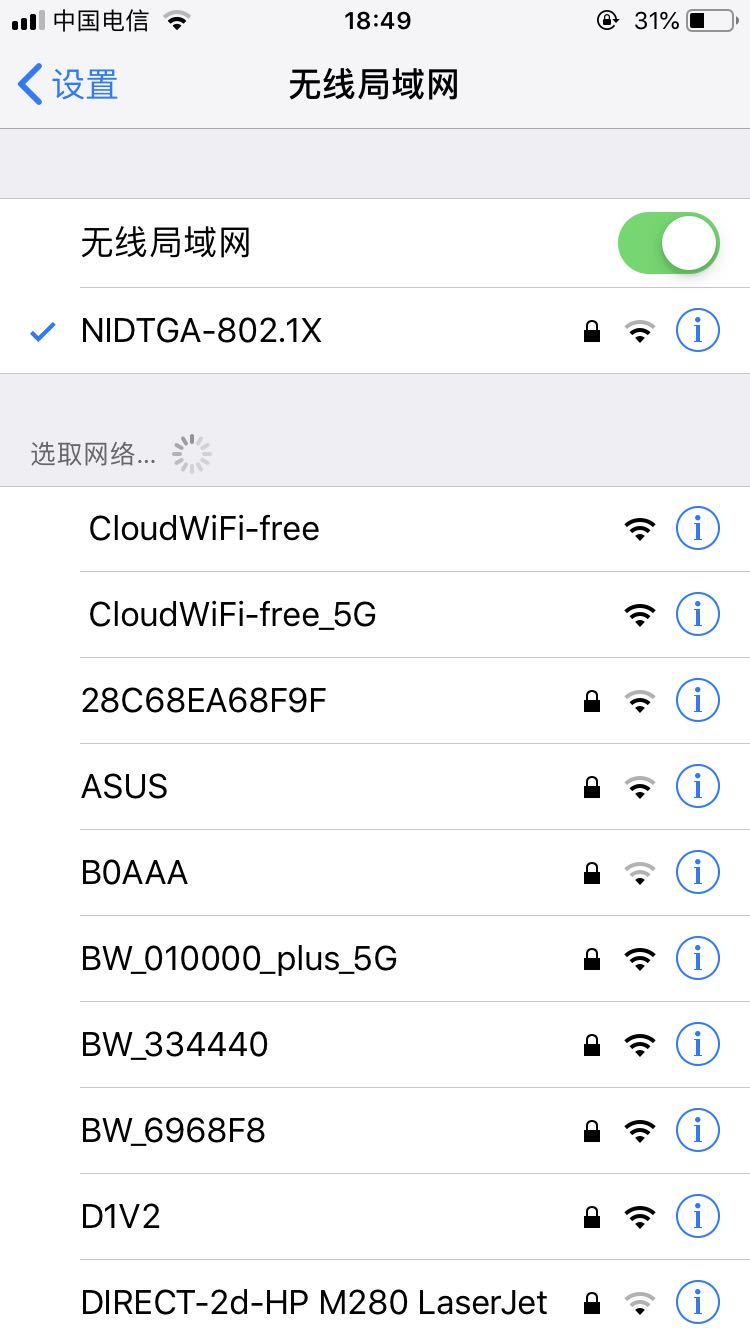
\includegraphics[height=6cm]{DHCPv6_8021X_deploy_1.jpeg}}
          \hspace{2em}
          \subcaptionbox{地址配置页面}
          {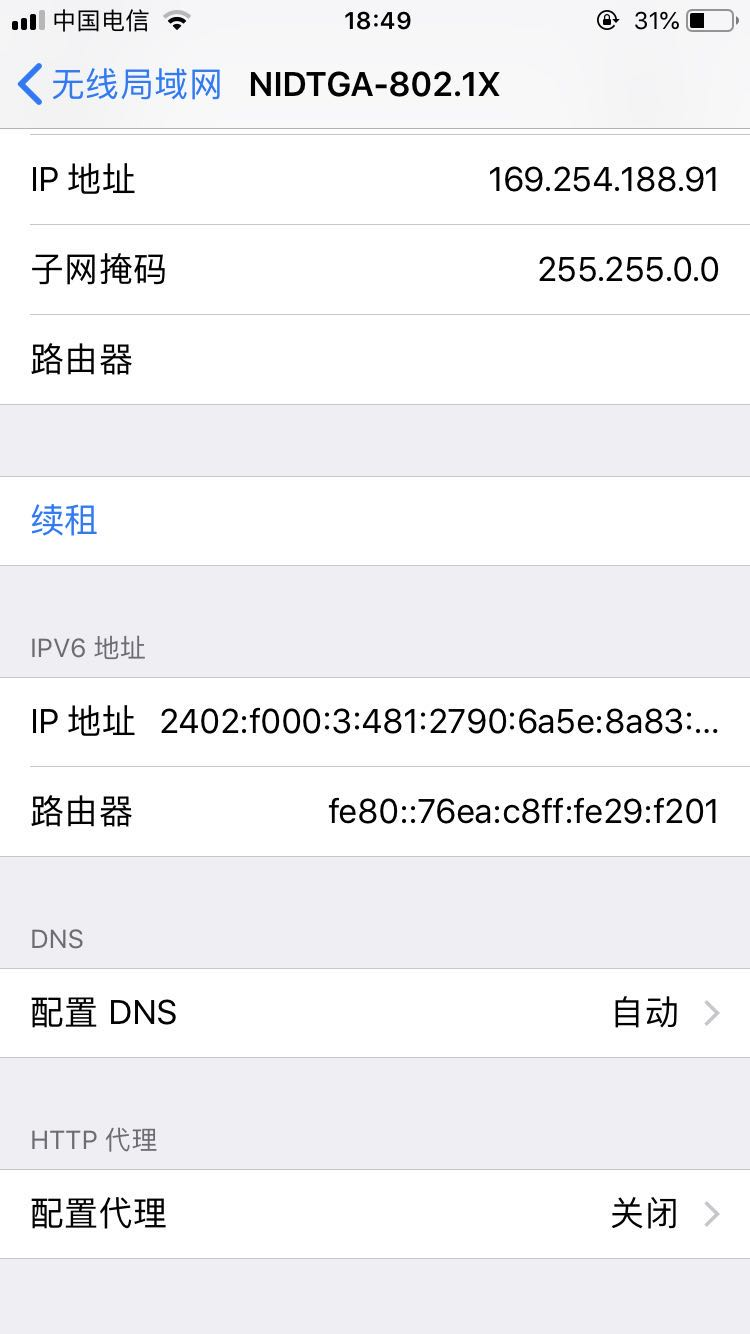
\includegraphics[height=6cm]{DHCPv6_8021X_deploy_2.jpeg}}
          \caption{清华大学二层准入认证系统部署用户认证举例}
          \label{fig:DHCPv6_8021X_deploy_result}
        \end{figure}
    
        目前,系统已在清华大学校园网中进行了部署与测试,在清华大学FIT楼104、204、229等房间的无线网络信号中有一个名为“NIDTGA-802.1X”的SSID。清华大学的师生连接该SSID后使用学校用户密码即可认证并访问网络。图\ref{fig:DHCPv6_8021X_deploy_result}所示为本文作者在iPhone手机上使用清华大学学生账号的用户名与密码连接“NIDTGA-802.1X”的页面举例,从第三张图中可以看到成功配置了一个由NIDTGA地址生成方案生成的IPv6地址。

    
    \subsection{三种系统设计方案的分析与对比}
    \label{NIDTGA:DHCPv6:comparison}
    在国家十三五重点研发项目“地址驱动的网络安全管控体系结构及其机理研究”中,DHCPv6下的用户身份识别与溯源系统将作为一项基础技术与应用示范在CNGI-CERNET2所连接的全国41所学校进行推广部署。本文在此分析各种认证方式下系统设计方案的优缺点,选择最适宜推广部署的方案总结在实际网络环境中的部署指南。
    
    三种方案在对用户设备、网络设备、系统实现等方面有着各自不同的要求,本文在此总结如下:
    \begin{enumerate}[1{)}]
      \item \textbf{扩展DHCPv6认证方案}:扩展DHCPv6认证方案需要禁用用户设备自身操作系统内核的DHCPv6客户端,使用自定义的DHCPv6客户端进行地址请求与配置,这种方式虽然可以支持一些暂不支持DHCPv6的操作系统,比如Android、Chrome OS等设备,但由于目前市场上操作系统繁杂,不同操作系统的系统调用接口均不同,同一操作系统的不同版本之间也存在差异,为了实现对用户设备的广泛支持,需要对每种操作系统进行针对性的客户端开发和维护,工作量巨大。对于Android等设备,安装定制DHCPv6客户端也需要用户拥有root权限,对用户并不友好。并且,采用扩展DHCPv6认证的方式,其认证过程与地址请求过程相耦合,虽然在本文的方案设计中采用了随机数的机制设计保护用户信息,但DHCPv6协议的安全问题仍会导致用户信息泄露、地址请求被假冒等问题。同时,在无线环境中,扩展DHCPv6认证手段本身无法保证用户认证后MAC地址不发生伪造,因此为了实现无线SAVI技术\cite{I-D.bi-savi-wlan},必须在网络中启用802.11i\cite{IEEE80211i}对MAC地址进行保护。在不使用802.1X认证的情况下,802.11i要求用户在接入网络时填写加密协商通信密钥过程的主密钥,这步密钥填写与用户采用定制的DHCPv6客户端的用户密码不同,可能令用户造成一定的困惑。
      \item \textbf{Web Portal认证方案}:Web Portal认证方案采用了轻量级的用户认证方式,用户设备无需安装任何客户端,使用浏览器即可以进行认证。其认证与地址配置流程均使用较为通用和标准化的技术,仅要求网络中接入控制设备具备对Web Portal认证功能的支持,但是该方案在DHCPv6服务器侧逻辑复杂,需要维护临时IPv6地址池与NIDTGA地址池的状态,在用户侧需要不断对临时IPv6地址进行续约,一方面会导致用户认证成功到用户获取得到NIDTGA地址之间存在一定延迟,影响用户体验,另一方面向网络中发送了大量的Renew报文,当用户数量较多时将显著增加网络设备负担。同时,通过Web Portal认证的方式也存在用户密码密文被窃取、用户身份被监听等安全隐患,需要HTTPS等协议的配合才能实现一定程度的安全性。同样,由于Web Portal认证手段无法保证用户MAC地址真实,因此在无线网络中也需要采用802.11i的机制以支持无线SAVI技术的部署。
      \item \textbf{二层准入认证方案}:二层准入认证方案的用户认证与地址配置方案均采用已被标准化的技术,对用户设备没有特殊要求,不需要安装客户端,也没有IPv6地址重新配置的流程,对用户比较友好,在DHCPv6服务器侧的状态维护比较简单。认证过程采用802.1X技术,可以保障认证过程中通信的安全性,并且防止攻击者伪造MAC地址,为无线SAVI技术的部署提供支持。地址配置过程中采用标准DHCPv6协议,对网络设备负担小。但是,由于需要向DHCPv6服务器告知请求地址的设备的MAC地址,因此该方案需要第一跳DHCPv6中继设备(一般是子网网关)支持RFC 6939这一标准。
    \end{enumerate}

    本文将三种方案的异同点总结如表\ref{tab:DHCPv6_implimentation_compare}所示。可见,二层准入认证的用户身份识别与溯源方案更为安全,认证过程对用户更友好,且对网络设备没有性能负担,原生支持无线SAVI的部署,保证用户源IPv6地址真实,适合推广部署。
    \begin{table}[htb]
      \centering
      \begin{minipage}[t]{\linewidth} 
        \caption{用户身份识别与溯源系统三种设计方案对比}
        \label{tab:DHCPv6_implimentation_compare}
        \begin{tabularx}{\linewidth}{c>{\centering\arraybackslash}X>{\centering\arraybackslash}X>{\centering\arraybackslash}X}
          \toprule[1.5pt]
          {\heiti 系统设计方案} & {\heiti 扩展DHCPv6认证} & {\heiti Web Portal认证} & {\heiti 二层准入认证} \\\midrule[1pt]
          {\heiti 用户设备要求} & 安装定制客户端 & 无 & 无 \\ 
          {\heiti 接入设备要求} & 无 & 无 & 802.1X认证 \\ 
          {\heiti 网关设备要求} & 无 & Web Portal认证 & DHCPv6 Client Link-Layer Address选项 \\ 
          {\heiti 地址分配过程} & 扩展DHCPv6,一次分配 & 标准DHCPv6,二次分配 & 标准DHCPv6,一次分配 \\  
          {\heiti 地址安全} & 无线网络中需要增加802.11i防止MAC地址伪造 & 无线网络中需要增加802.11i防止MAC地址伪造 & 原生支持MAC地址真实 \\
          {\heiti 优点} & 用户认证与地址配置流程简单,租约管理容易,可以支持没有DHCPv6功能的设备 & 无需用户安装客户端 & 无需用户安装客户端,认证过程安全且对用户友好,地址配置流程简单,租约管理容易 \\ 
          {\heiti 缺点} & 用户需要安装定制客户端,客户端需适配各操作系统版本开发并定期升级维护;需要用户填写802.11i加密密钥,对用户不友好;认证过程不安全 & 地址配置流程复杂;用户地址获取存在延迟;网络设备压力大;对网关设备有支持Web Portal认证的特殊需求;无法支持没有DHCPv6功能的设备;需要用户填写802.11i加密密钥,对用户不友好 & 对网关设备有支持DHCPv6 RFC6939的特殊需求;无法支持没有DHCPv6功能的设备 \\ 
          \bottomrule[1.5pt]
        \end{tabularx}
      \end{minipage}
    \end{table}

    \subsection{二层准入认证系统的校园网部署方案}
    \label{NIDTGA:DHCPv6:deploy}
    \ref{NIDTGA:DHCPv6:comparison}节中比较了多种用户身份识别与溯源系统的设计方案,并分析指出了基于二层准入认证的方案最为安全且用户友好。在对其进行实现后,如何在实际网络环境中部署也是用户身份识别与溯源系统得到实际应用至关重要的一环。由于支持DHCPv6配置地址的设备既有通过无线网络连接的笔记本、非Android操作系统的手机等移动终端,也有通过有线网络连接的台式电脑、服务器等设备,因此本节以校园网络为例,分别对无线与有线的两种环境下的部署方案进行研究。

      \subsubsection{无线校园网}
      \label{NIDTGA:DHCPv6:deploy:wireless}
      在CNGI-CERNET2所连接的41所全国高等院校中,所有学校的无线网络主要组网方式均为基于无线控制器的架构,尽管这种架构下对于802.1X报文等来自用户的管理帧均统一发送到AC进行处理,但对于用户的数据帧存在两种不同的报文转发模式:
      \begin{enumerate}[1{)}]
        \item \textbf{本地转发}:数据报文到达AP后,无需经过AC,直接由AP转发至上层网络经由有线网关进行路由转发。
        \item \textbf{集中转发}:数据报文到达AP后,由AP进行封装,统一经过IP隧道到达AC,由AC解封装后进行路由转发。
      \end{enumerate}

      根据\ref{NIDTGA:DHCPv6:comparison}节的分析,二层准入认证的用户身份识别与溯源系统对网络设备的功能有所要求,需要在用户设备经过的第一跳DHCPv6中继处支持RFC 6939中定义的Client Link-Layer Address选项以在Relay Forward报文中携带用户设备MAC地址。在本地转发模式下,第一跳DHCPv6中继为有线网关设备,而在集中转发模式下,第一跳DHCPv6中继为AC所旁挂的核心路由器设备。此外,由于实现用户身份识别与溯源的前提是IPv6地址真实,因此必须保证用户获取NIDTGA地址后访问网络时所使用的地址确实为其获取的NIDTGA地址,而非用户随意伪造的IPv6地址,因此用户身份识别与溯源系统还要求部署区域必须采用SAVI技术。

      因此,设计两种转发模式下的部署要求如图\ref{fig:wireless_deploy_request}所示。本地转发时的配置如下:
      \begin{itemize}
        \item AC:为用户身份识别与溯源系统划分出独立的SSID,配置相应VLAN、本地转发模式;配置接入子网源地址验证的SAVI技术,开启DHCPv6 Snooping;配置802.1X的认证方式,并设置AAA服务器地址、与AAA服务器进行通信的密钥等信息。
        \item AP上连的有线网关:为部署用户身份识别与溯源系统的VLAN开启DHCPv6中继功能,设置DHCPv6服务器地址,开启DHCPv6 Client Link-Layer Address选项功能;配置RA报文,开启Managed位与Other位,关闭Autonomous位。有线网关根据组网方式的不同可能位于汇聚交换机或核心路由器上,图\ref{fig:wireless_deploy_request}中以汇聚交换机为有线网关示意。
      \end{itemize}

      集中转发模式下的部署要求如下:
      \begin{itemize}
        \item AC:为用户身份识别与溯源系统划分出独立的SSID,配置相应VLAN、集中转发模式;配置SAVI,开启DHCPv6 Snooping;配置802.1X的认证方式,并设置AAA服务器地址、与AAA服务器进行通信的密钥等信息。
        \item AC所旁挂的核心路由器:为部署用户身份识别与溯源系统的VLAN开启DHCPv6中继功能,设置DHCPv6服务器地址,开启DHCPv6 Client Link-Layer Address选项功能;配置RA报文,开启Managed位与Other位,关闭Autonomous位。
      \end{itemize}

      \begin{figure}[ht]
        \centering
        \subcaptionbox{无线校园网部署拓扑\label{fig:wireless_deploy_request}}
        {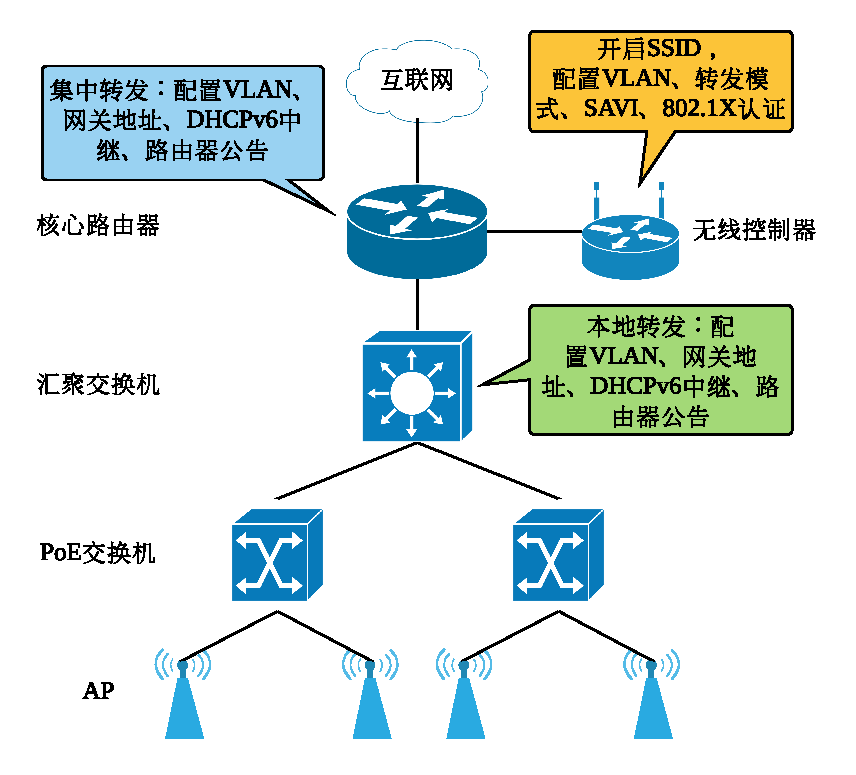
\includegraphics[height=5cm]{wireless_deploy_request.pdf}}
        \hspace{2em}
        \subcaptionbox{有线校园网部署拓扑\label{fig:wired_deploy_request}}
        {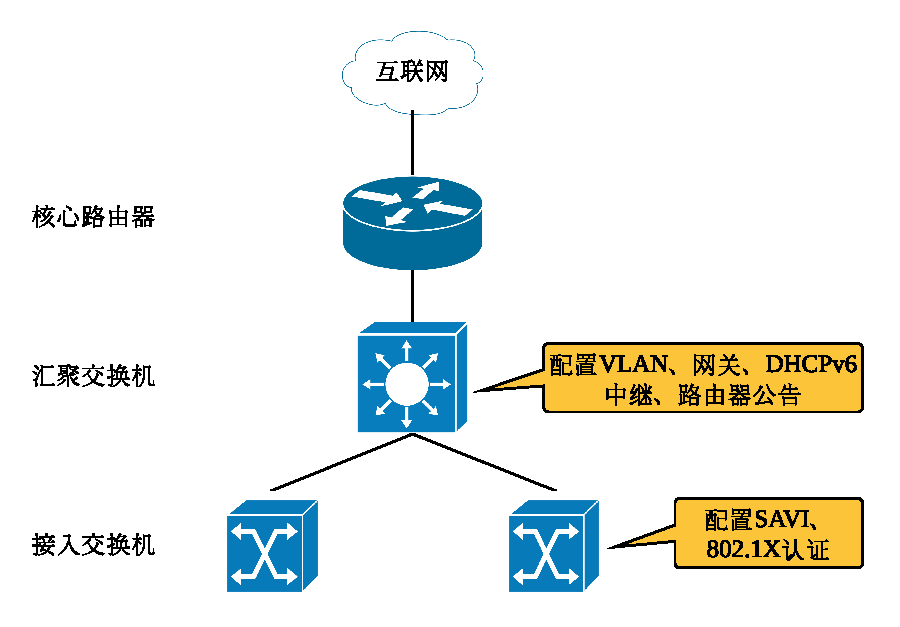
\includegraphics[height=5cm]{wired_deploy_request.pdf}}
        \caption{校园网部署拓扑示意}
      \end{figure}

      \subsubsection{有线校园网}
      \label{NIDTGA:DHCPv6:deploy:wired}
      有线校园网络的典型拓扑较为简单,一般为用户设备连接在接入交换机上,接入交换机上连汇聚交换机,汇聚交换机再连接至校园网的核心路由器上。有线网关的位置根据管理方式的不同可能位于汇聚交换机上,也可能位于核心路由器上。其部署的要求如图\ref{fig:wired_deploy_request}所示:
      \begin{itemize}
        \item 接入交换机:对用户接入端口配置802.1X认证,设置AAA服务器地址、通信密钥等,并配置SAVI功能,开启DHCPv6 Snooping;
        \item 有线网关设备:为用户身份识别与溯源系统的部署区域划分VLAN;为部署的VLAN开启DHCPv6中继功能,设置DHCPv6服务器地址,开启DHCPv6 Client Link-Layer Address选项功能;配置RA报文,开启Managed与Other位,关闭Autonomous位。
      \end{itemize}

      \subsubsection{部署方案总结}
      \label{NIDTGA:DHCPv6:deploy:summary}
      由于各个高校的组网方式互相之间存在一些差异,尽管在前两小节对具有共性的组网方案进行了描述,但为了在实际推广部署时根据高校网络具体情况因地制宜提供指导,本文在此总结部署用户身份识别与溯源系统的需求框架。
      在无线网络与有线网络中进行部署时,有一些共同的要求:
      \begin{enumerate}[1{)}]
        \item \textbf{设备部署}:部署用户身份识别与溯源系统需要在校园网中添加技术相关的自研设备,包括采用NIDTGA地址生成方式的DHCPv6服务器、用户认证的AAA服务器,两个服务器均需要稳定的有线接入,配置静态的不发生变化的IPv6地址。
        \item \textbf{子网划分}:网络中需要划分部署用户身份识别与溯源系统的用户接入子网与部署系统控制设备的系统控制子网。每一个用户接入子网应独享一个/64的IPv6前缀,以确保用户设备可以正常获取和使用NIDTGA地址。系统控制子网需与用户接入子网保持独立,不与任何用户设备处于同一子网内,以确保用户设备发送的DHCPv6报文经过DHCPv6中继以携带Client Link-Layer Address选项。
      \end{enumerate}

      不论是有线环境还是无线环境,用户身份识别与溯源系统的部署对网络中已有设备的要求是一致的,只是根据组网方式的不同,DHCPv6中继与802.1X接入控制设备的位置在网络中会有所变化,本文将各种组网方式下行使各功能的网络设备与配置要求总结如表\ref{tab:DHCPv6_deploy_summary}所示。

      \begin{table}[htb]
        \centering
        \begin{minipage}[t]{\linewidth} 
          \caption{DHCPv6不同组网方式下的网络设备位置与配置要求总结}
          \label{tab:DHCPv6_deploy_summary}
          \begin{tabularx}{\linewidth}{>{\centering}m{2cm}>{\centering}m{1.8cm}>{\centering}m{1.8cm}>{\centering}m{1.8cm}>{\centering\arraybackslash}X}
            \toprule[1.5pt]
            \multirow{2}{*}{\heiti 设备功能} & \multicolumn{3}{c}{\heiti 组网方式} & \multirow{2}{*}{\heiti 配置要求} \\ 
            & {\heiti 无线网络本地转发} & {\heiti 无线网络集中转发} & {\heiti 有线网络} & \\\midrule[1pt]
            {\heiti 接入设备} & AP & AP & 接入交换机 & 开启SAVI,DHCPv6 Snooping \\ 
            {\heiti 802.1X接入控制设备} & AC & AC & 接入交换机 & 配置802.1X认证,设置AAA服务器地址与通信密钥  \\ 
            {\heiti DHCPv6中继} & 有线网关设备 & AC旁挂设备 & 有线网关设备 & 开启中继,设置DHCPv6服务器地址,开启Client Link-Layer Address选项功能  \\ 
            {\heiti 子网网关} & 汇聚交换机或核心路由器 & 核心路由器 & 汇聚交换机或核心路由器 & 划分VLAN,配置网关地址、IPv6前缀,开启路由器公告报文中Managed与Other位,关闭Autonomous位 \\
            \bottomrule[1.5pt]
          \end{tabularx}
        \end{minipage}
      \end{table}

  \section{SLAAC下的用户身份识别与溯源系统}
  \label{NIDTGA:SLAAC}
  尽管DHCPv6的地址配置方式更有利于组织管理员对用户上网进行控制和管理,但其地址配置流程比无状态地址配置SLAAC方式更为复杂,并且目前仍有设备的操作系统未实现DHCPv6协议,如Android系统、Chrome OS系统等,因此SLAAC方式仍是IPv6网络中一种重要的地址配置方式。

  但是,SLAAC方式由用户设备生成IPv6地址并进行重复地址检测,组织管理员无法控制用户如何生成和使用某一特定IPv6地址。同样,因为不能将IDEA密钥分发到用户端用于地址的生成,所以也不能通过类似于DHCPv6方式下定制客户端的方式实现。即便将密钥下发到用户端,也无法防止恶意用户使用错误的密钥或加密方式生成IPv6地址。

  SDN-Ti\cite{SDNTi}提出使用SDN对SLAAC地址配置方式下的用户IPv6地址进行映射,由SDN控制器为用户生成NIDTGA地址并下发映射规则给SDN交换机,SDN交换机负责将用户数据报文中的源IPv6地址替换为用户对应的NIDTGA地址再进行向外的转发,同时对以用户NIDTGA地址为目的地址的报文将其目的地址替换为用户设备的SLAAC地址后向内转发。SDN-Ti本质上是对用户使用SLAAC配置的IPv6地址进行了NAT,其虽然提出了SLAAC配置下实现用户身份识别与溯源系统的一种解决方案,但其在部署时需要将SDN交换机部署至每一个AP之上,SDN控制器也需要与AC协同工作处理所有的报文,这将极大地影响非通过用户身份识别与溯源系统接入的网络流量,容易造成网络的拥塞与不稳定,严重影响其他网络接入服务的可用性,其弊端大于配置NIDTGA地址的优势。

  因此,本文仍采用身份绑定的方式实现用户身份的溯源功能,作为覆盖暂未支持DHCPv6功能的设备的折中方案,而不将NID嵌入用户的IPv6地址中。

    \subsection{用户身份识别与溯源系统整体架构}
    \label{NIDTGA:SLAAC:architecture}
    本文设计的SLAAC地址配置方式下用户身份识别与溯源系统包含如图\ref{fig:SLAAC_system_architecture}所示的几个主要组成部分:
    \begin{enumerate}[1{)}]
      \item \textbf{认证控制设备}:网络中对用户接入进行认证控制的网络设备,一般为AC、接入交换机或宽带接入服务器等。用户所有流量均通过认证控制设备后才能进行跨子网的转发,认证控制设备将根据用户设备的认证情况,决定用户流量的转发策略。
      \item \textbf{SAVI设备}:监听用户设备地址配置控制报文的SAVI设备,将生成的IPv6地址与MAC地址等绑定表上报给认证管理服务器,一般部署于用户设备与认证控制设备之间,或者与认证控制设备一体。
      \item \textbf{认证管理服务器}:保存用户认证数据库的服务器。根据网络中认证手段的不同,具体形式将发生变化,在Web Portal认证方式下将包含Web Portal服务器与AAA服务器;在二层准入认证时为AAA服务器。
      \item \textbf{追溯服务器}:保存IPv6地址与用户身份绑定信息历史、提供用户身份溯源功能的服务器。根据网络中认证手段的不同,在Web Portal认证时其IPv6地址与用户身份绑定信息直接由认证管理服务器上传;在二层准入认证时需要将认证管理服务器上传的用户认证信息与SAVI设备上传的SAVI表项相结合,进行IPv6地址与用户身份绑定项的生成。
    \end{enumerate}

    \begin{figure}[ht]
      \centering
      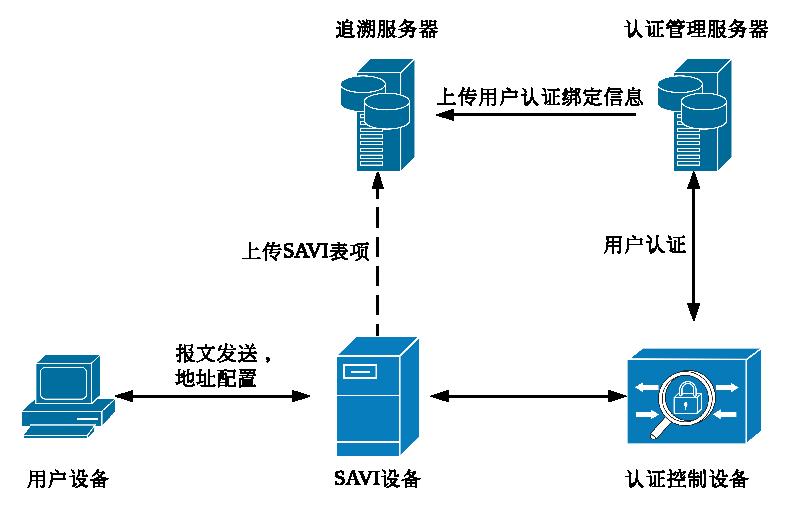
\includegraphics[width=0.7\textwidth]{SLAAC_system_architecture.pdf}
      \caption{SLAAC下用户身份识别与溯源系统整体架构}
      \label{fig:SLAAC_system_architecture}
    \end{figure}

    在用户通过用户身份识别与溯源系统接入网络时,根据网络中配置的认证手段不同,在Web Portal认证下用户设备将先通过SLAAC配置地址再发起用户身份认证,在二层准入认证时则先完成用户身份认证而后配置IPv6地址。前者由于认证时设备已经配置了IPv6地址,因此可以较为简单地进行IP地址与用户身份的绑定;后者由于认证时设备尚未配置IPv6地址,因此本文提出了一种利用设备MAC地址标识设备、认证与SAVI技术相配合完成IPv6地址与用户身份绑定的设计方案。

    \subsection{基于Web Portal认证的系统设计}
    \label{NIDTGA:SLAAC:portal}
    在Web Portal认证的方式下,用户的NID与IPv6地址的关系可以在用户登录Web Portal认证的过程中比较容易地获取,其认证过程如图\ref{fig:SLAAC_web_portal}所示:
    \begin{enumerate}[1{)}]
      \item 网关向用户设备发送路由器公告RA报文,包含可配置的IPv6前缀等信息;
      \item 用户设备生成IPv6前缀下的IPv6地址后进行重复地址检测;
      \item 若用户设备在等待时间内未收到其他节点发来的对相同IPv6地址进行重复地址检测的NS报文或宣告持有该IPv6地址的邻居公告NA报文,则重复地址检测成功,设备为其网络接口配置该IPv6地址,并设定网关地址等信息;
      \item 用户使用浏览器访问网络,认证设备处还未有该IPv6地址的流量处理规则,因此被重定向至Web Portal网址;
      \item 用户提交NID与密码至Web Portal网站,Web Portal系统校验成功后,将用户NID与IPv6地址、认证时间信息上送给追溯服务器,并下发流量放行规则给认证控制设备;
      \item 认证控制设备允许用户数据报文正常转发;
      \item 用户手动访问Web Portal网站进行下线或认证控制设备检测到用户一段时间没有流量时,Web Portal认证系统向追溯服务器上传IPv6地址与下线时间。
    \end{enumerate}

    \begin{figure}[ht]
      \centering
      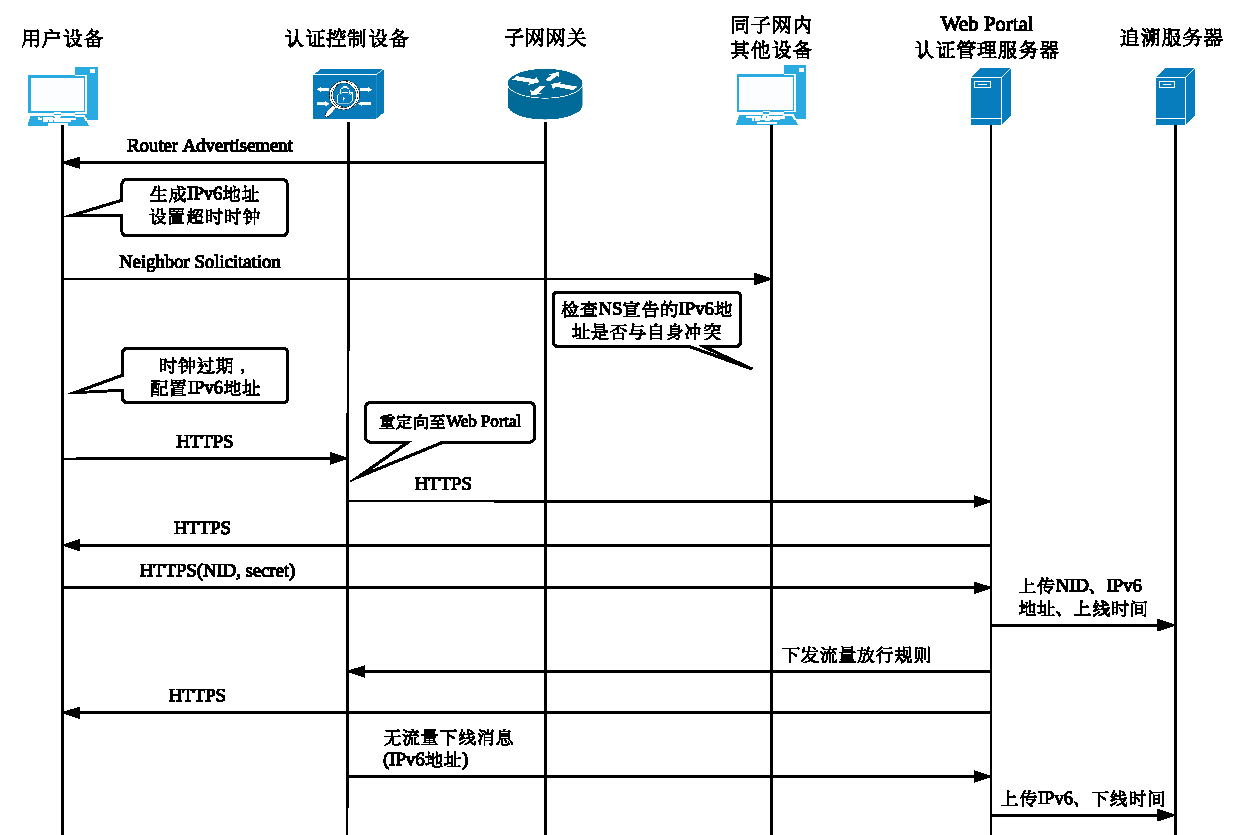
\includegraphics[width=0.9\textwidth]{SLAAC_web_portal.pdf}
      \caption{SLAAC下Web Portal认证的用户身份识别与溯源系统时序}
      \label{fig:SLAAC_web_portal}
    \end{figure}

    追溯服务器在收到Web Portal认证管理服务器上传的用户认证信息后,需要将NID、IPv6地址、时间等记录在数据库中,以供追溯使用,其表结构如\ref{tab:SLAAC_web_portal_binding}所示。
    \begin{table}[htb]
      \centering
      \begin{minipage}[t]{\linewidth} 
        \caption{SLAAC下Web Portal认证绑定关系数据表}
        \label{tab:SLAAC_web_portal_binding}
        \begin{tabularx}{\linewidth}{>{\centering\arraybackslash}X>{\centering\arraybackslash}X>{\centering\arraybackslash}X>{\centering\arraybackslash}X}
          \toprule[1.5pt]
          {\heiti 用户NID} & {\heiti IPv6地址} & {\heiti 上线时间} & {\heiti 下线时间}  \\\midrule[1pt]
          80002888b1 & 2402:f000:6:1c01: 6c28:70f1:be03:efe6 & 1583754484 & 1583758084 \\ 
          \multicolumn{4}{c}{...} \\
          \bottomrule[1.5pt]
        \end{tabularx}
      \end{minipage}
    \end{table}

    \subsection{基于二层准入认证的系统设计}
    \label{NIDTGA:SLAAC:8021X}
    在二层准入认证方式下,由于用户先使用链路层协议完成认证,后通过SLAAC配置IPv6地址,因此难以在用户认证时对用户NID与IPv6地址进行关联。考虑到用户身份识别与溯源系统所依赖的接入子网源地址验证技术SAVI能够监听SLAAC配置时的重复地址检测过程,并将无线网络中的信任锚MAC地址与IPv6地址进行绑定,而802.1X认证时同样以MAC地址标识不同的设备,因此我们可以采用MAC地址作为桥梁将用户NID与IPv6地址进行关联。

    本文在追溯服务器处维护已认证设备表与SAVI绑定表,分别如表\ref{tab:SLAAC_authorized_devices}与表\ref{tab:SLAAC_savi}所示,并根据两表通过算法\ref{algo:nid_ipv6_binding_table}生成用户身份与IPv6地址绑定表,如表\ref{tab:SLAAC_NID_IPv6_binding}所示。此外,追溯服务器还将生成已下线用户绑定表并写入数据库中,以支持对历史用户NID的查询。

    \begin{table}[htb]
      \centering
      \begin{minipage}[t]{\linewidth} 
        \caption{已认证设备表}
        \label{tab:SLAAC_authorized_devices}
        \begin{tabularx}{\linewidth}{>{\centering\arraybackslash}X>{\centering\arraybackslash}X>{\centering\arraybackslash}X}
          \toprule[1.5pt]
          {\heiti 设备MAC} & {\heiti 用户NID} & {\heiti 认证时间}  \\\midrule[1pt]
          78:31:c1:c8:10:8c & 80002888b1 & 1583754484 \\ 
          \multicolumn{3}{c}{...} \\
          \bottomrule[1.5pt]
        \end{tabularx}
      \end{minipage}
    \end{table}

    \begin{table}[htb]
      \centering
      \begin{minipage}[t]{\linewidth} 
        \caption{SAVI绑定表}
        \label{tab:SLAAC_savi}
        \begin{tabularx}{\linewidth}{>{\centering\arraybackslash}X>{\centering\arraybackslash}X>{\centering\arraybackslash}X}
          \toprule[1.5pt]
          {\heiti 设备MAC} & {\heiti AP} & {\heiti IPv6地址列表} \\\midrule[1pt]
          78:31:c1:c8:10:8c & 30-7B-AC-93-27-80: NIDTGA-802.1X & 2402:f000:6:1c01: 6c28:70f1:be03:efe6 \\ 
          \multicolumn{3}{c}{...} \\
          \bottomrule[1.5pt]
        \end{tabularx}
      \end{minipage}
    \end{table}

    \begin{table}[htb]
      \centering
      \begin{minipage}[t]{\linewidth} 
        \caption{在线用户绑定表}
        \label{tab:SLAAC_NID_IPv6_binding}
        \begin{tabularx}{\linewidth}{>{\centering\arraybackslash}X>{\centering\arraybackslash}X>{\centering\arraybackslash}X>{\centering\arraybackslash}X}
          \toprule[1.5pt]
          {\heiti 设备MAC} & {\heiti 用户NID} & {\heiti IPv6地址列表} & {\heiti 认证时间}\\\midrule[1pt]
          78:31:c1:c8:10:8c & 80002888b1 & 2402:f000:6:1c01: 6c28:70f1:be03:efe6 & 1583754484 \\ 
          \multicolumn{4}{c}{...} \\
          \bottomrule[1.5pt]
        \end{tabularx}
      \end{minipage}
    \end{table}

    其中表\ref{tab:SLAAC_authorized_devices}根据设备认证情况实时更新,每当有设备上线或下线时,AAA服务器将告知追溯服务器相应的用户NID与MAC地址信息,追溯服务器即将相应表项进行插入或删除。表\ref{tab:SLAAC_savi}则由认证控制设备在每当有新的SAVI绑定表项更新时上送给追溯服务器。

    \begin{algorithm}[ht]
      \caption{NID与IPv6地址绑定表生成算法}
      \label{algo:nid_ipv6_binding_table}
      
      \LinesNumbered
      \SetKw{KwInList}{in}
      \SetKw{KwBreak}{break}
      \KwIn{authorized\_device\_table, SAVI\_binding\_table}
      \KwOut{NID\_IPv6\_binding\_table}

      NID\_IPv6\_binding\_table \gets empty list\;
      \For{(MAC, NID, auth\_time) \KwInList authorized\_device\_table}{
        \For{(savi\_MAC, AP, IPv6\_list) \KwInList SAVI\_binding\_table}{
          \If{MAC $==$ savi\_MAC} {
            NID\_IPv6\_binding\_table.add((MAC, NID, IPv6\_list, auth\_time))\;
            \KwBreak\;
          }
        }
      }
    \end{algorithm}

    \begin{algorithm}[ht]
      \caption{已下线用户生成算法}
      \label{algo:nid_ipv6_logout_user}
      
      \LinesNumbered
      \SetKw{KwInList}{in}
      \SetKw{KwBreak}{break}
      \SetKw{KwTrue}{true}
      \SetKw{KwFalse}{false}
      \SetKw{KwAnd}{and}
      \KwIn{old\_NID\_IPv6\_binding\_table, new\_NID\_IPv6\_binding\_table}
      \KwOut{logout\_users}

      logout\_users \gets empty list\;
      \For{(old\_MAC, old\_NID, old\_IPv6\_list, old\_auth\_time) \KwInList old\_NID\_IPv6\_binding\_table}{
        is\_logout \gets \KwTrue\;
        \For{(new\_MAC, new\_NID, new\_IPv6\_list, new\_auth\_time) \KwInList new\_NID\_IPv6\_binding\_table}{
          \If{old\_NID $==$ new\_NID \KwAnd old\_IPv6\_list $==$ new\_IPv6\_list} {
            is\_logout \gets \KwFalse\;
            \KwBreak\;
          }
        }
        \If{is\_logout} {
          logout\_users.add((old\_MAC, old\_NID, old\_IPv6\_list, old\_auth\_time, current\_time))\;
        }
      }
    \end{algorithm}

    表\ref{tab:SLAAC_NID_IPv6_binding}将在表\ref{tab:SLAAC_authorized_devices}与表\ref{tab:SLAAC_savi}发生更新时调用算法\ref{algo:nid_ipv6_binding_table}进行更新。生成最新的在线用户绑定表后,与更新前的在线用户绑定表相比较,根据算法\ref{algo:nid_ipv6_logout_user}获得已下线用户绑定表并写入数据库中,其结构如表\ref{tab:SLAAC_NID_IPv6_logout_users}所示。

    \begin{table}[htb]
      \centering
      \begin{minipage}[t]{\linewidth} 
        \caption{已下线用户绑定表}
        \label{tab:SLAAC_NID_IPv6_logout_users}
        \begin{tabularx}{\linewidth}{>{\centering\arraybackslash}Xc>{\centering\arraybackslash}Xcc}
          \toprule[1.5pt]
          {\heiti 设备MAC} & {\heiti 用户NID} & {\heiti IPv6地址列表} & {\heiti 上线时间} & {\heiti 下线时间}\\\midrule[1pt]
          78:31:c1:c8:10:8c & 80002888b1 & 2402:f000:6:1c01: 6c28:70f1:be03:efe6 & 1583754484 & 1583758679 \\ 
          \multicolumn{5}{c}{...} \\
          \bottomrule[1.5pt]
        \end{tabularx}
      \end{minipage}
    \end{table}
    

    用户认证上线的交互时序如图\ref{fig:SLAAC_802.1X}所示,详细步骤不再赘述。

    \begin{figure}[ht]
      \centering
      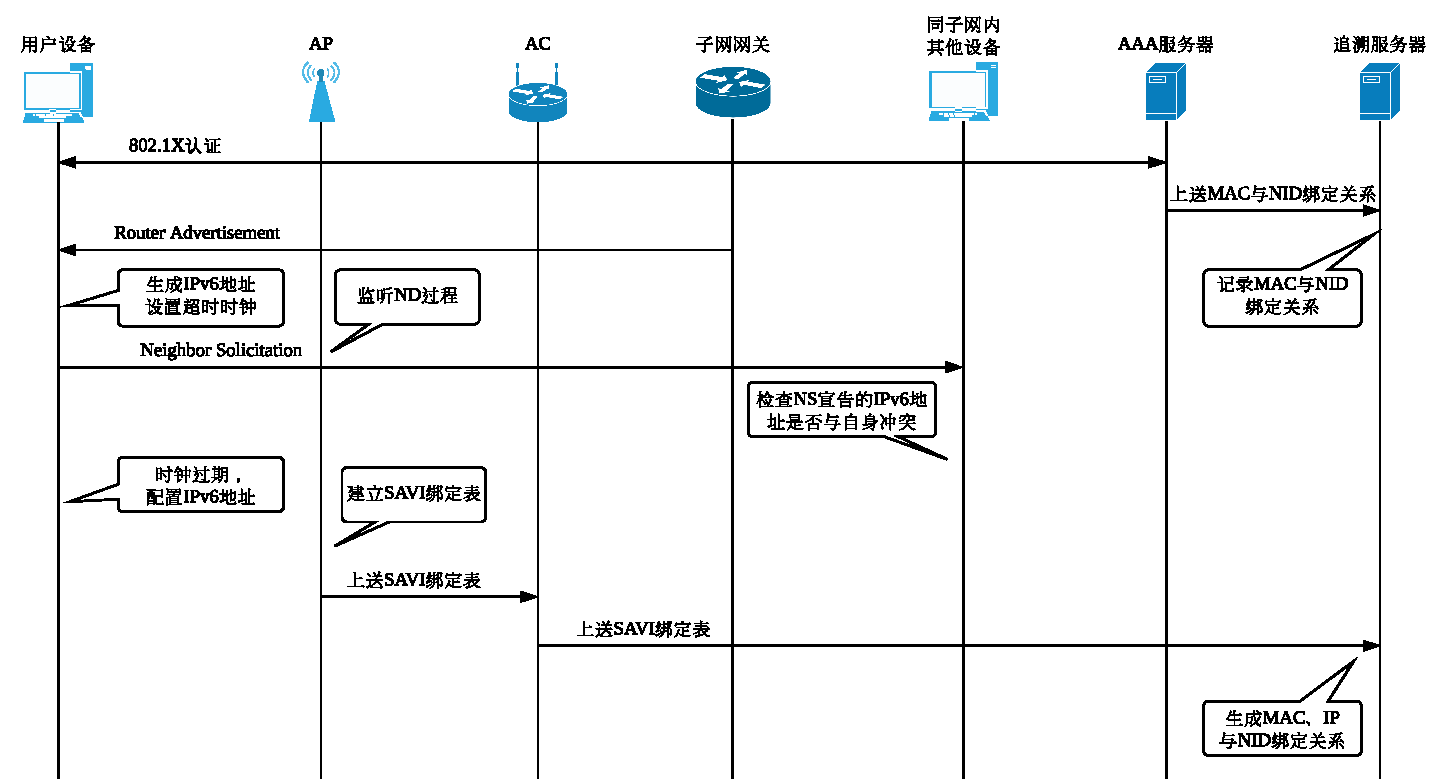
\includegraphics[width=0.9\textwidth]{SLAAC_8021X.pdf}
      \caption{SLAAC下二层准入认证的用户身份识别与溯源系统时序}
      \label{fig:SLAAC_802.1X}
    \end{figure}

    当有用户追溯请求时,即可以IPv6地址为关键字向数据库中已下线用户绑定表查询绑定的用户NID信息。

    \subsection{两种系统设计方案的分析与对比}
    \label{NIDTGA:SLAAC:comparison}
    用户身份识别与溯源系统的这两种设计均是对SLAAC配置方式下无法控制IPv6地址生成这一困境的折中选择,在未来所有主流用户设备均支持DHCPv6地址配置时将逐步避免在SLAAC下部署用户身份识别与溯源系统方案。由于有线接入的用户设备基本均支持DHCPv6配置地址,因此这两种方案应主要考虑在无线场景下的部署,以对Android手机等设备进行支持。

    从身份与IPv6地址的绑定流程上来看,基于Web Portal认证的方式更为简洁,也是目前大多数未采用用户身份识别与溯源系统的网络中对用户身份进行管理所采用的方案,但其缺少对MAC地址安全性的保证,因而需要额外增加802.11i的机制来支持无线SAVI技术的部署,需要用户填写链路加密密钥的过程可能对用户产生困扰。

    与Web Portal认证的方案相比,二层准入认证的方案由于采用802.1X认证,提供了无线SAVI技术所要求的MAC地址安全性保证,因此能够预防恶意用户同时伪造MAC地址与IPv6地址的情况。同时,由于其二层认证的特性,追溯服务器能够在用户认证时获取到标识用户设备的MAC地址,为整个用户身份识别系统增加了更多拓展的可能。比如,虽然802.1X能够防止用户在认证成功后重新伪造MAC地址,但是对于恶意用户在认证前修改了其他用户的MAC进行认证这种行为,认证系统无法进行判断。而在二层准入认证方案的追溯服务器中,追溯服务器可以获得所有AC上送的全网的用户信息,因而能够检测到MAC地址冲突的情况,对于恶意用户修改他人MAC地址进行认证造成MAC地址冲突影响网络体验的行为,其可以采取一些黑名单的制度,告知认证控制设备对恶意用户进行下线处理,以惩戒恶意用户的攻击行为,在SAVI技术保障IPv6地址真实的基础上提供MAC地址真实性的保证。

    \subsection{系统实现情况与校园网部署方案}
    \label{NIDTGA:SLAAC:deploy}
    不论是Web Portal认证还是二层准入认证下的系统设计方案,其均需要与认证控制设备、SAVI设备等网络设备相配合进行实现,因此需要与具体的网络设备厂商进行合作。

    目前,考虑到对移动设备的漫游支持,基于二层准入认证并增加了MAC地址冲突检测的安全增强方案已与华为、新华三厂商分别合作进行了实现,并在清华大学无线网络中进行了大规模部署。两者的实现方案如图\ref{fig:Tsinghua_SAVI_implementation}所示。其中华为的Agile Controller与新华三的地址安全中心将记录全量的用户五元组信息绑定表并存储于清华大学大数据平台,在用户认证时提供全局的MAC地址、IPv6地址冲突校验功能,并与无线控制器进行通信将非法的用户设备进行下线处理。值得注意的是,两者的方案是建立在SAVI技术提供的源地址真实性基础上的源地址验证与溯源基础设施,其对MAC地址、IPv6地址进行冲突校验的功能不与IPv6地址配置方式耦合,因此同样适用于\ref{NIDTGA:DHCPv6:8021X}节中提出的系统设计方案,可为其提供MAC地址冲突校验的增强性保障。
    
    \begin{figure}[ht]
        \centering
        \subcaptionbox{华为IPv6源地址溯源方案\label{fig:Tsinghua_SAVI_huawei}}
        {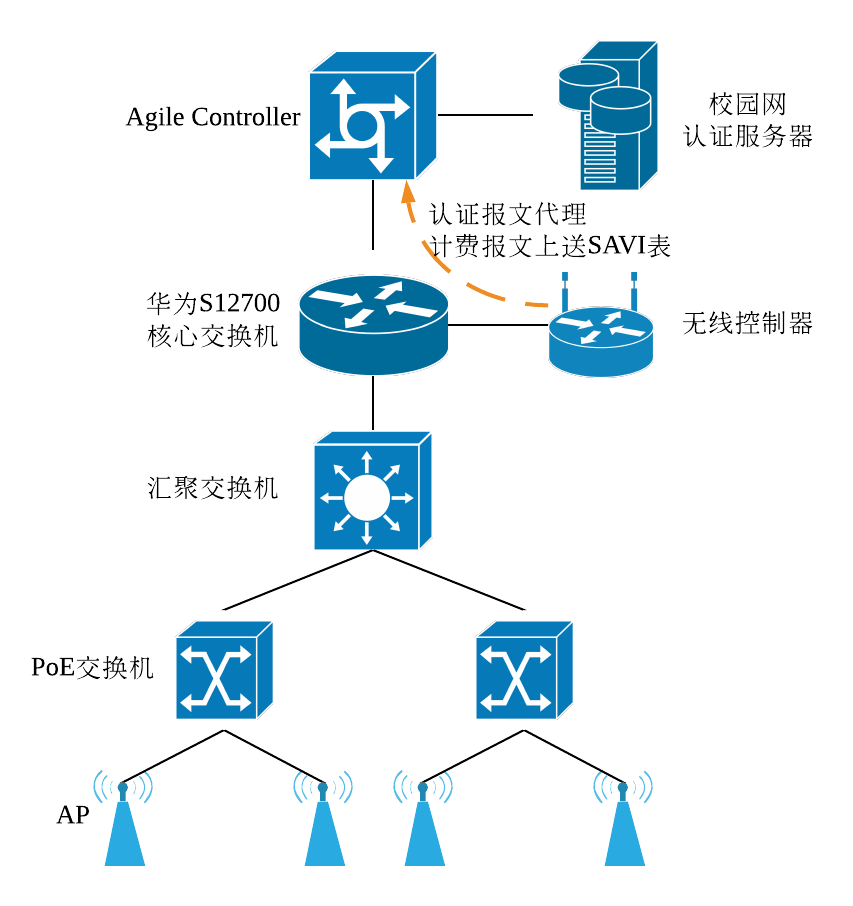
\includegraphics[height=7cm]{figures/Tsinghua_SAVI_huawei.png}}
        \subcaptionbox{新华三IPv6源地址溯源方案\label{fig:Tsinghua_SAVI_h3c}}
        {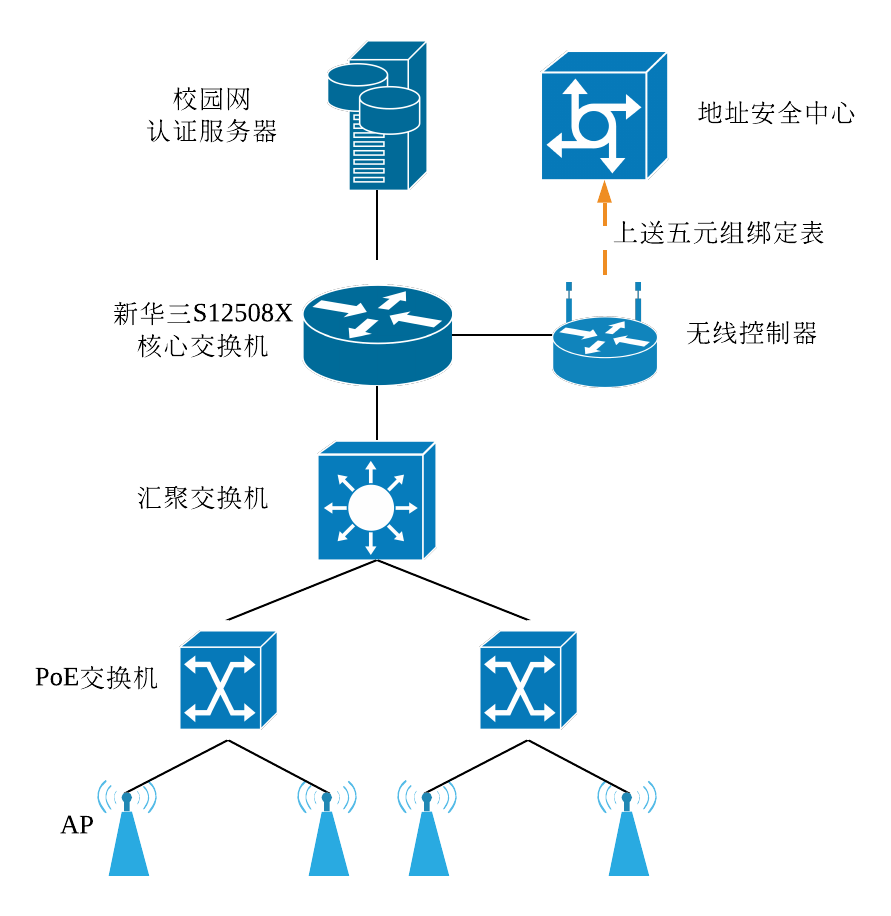
\includegraphics[height=7cm]{figures/Tsinghua_SAVI_h3c.png}}
        \caption{SLAAC下用户身份识别与溯源系统的厂商实现与部署方案示意}
        \label{fig:Tsinghua_SAVI_implementation}
    \end{figure}

    由于用户身份识别与溯源系统在SLAAC下的设计方案均采用了被广泛应用或已标准化的认证技术与地址配置手段,用户身份与IPv6绑定都在服务器侧通过扩展功能实现,因此对于网络中的部署没有特殊的要求,各自采用传统的Web Portal认证与802.1X认证的部署方案即可。此外,同样需要网络设备采用SLAAC地址配置下的SAVI技术对用户伪造源IPv6地址的流量进行过滤,确保只有真实IPv6地址的流量才能够访问网络。本文将对各网络设备的要求总结如表\ref{tab:SLAAC_deploy_summary}所示。
    \begin{table}[htb]
      \centering
      \begin{minipage}[t]{\linewidth} 
        \caption{SLAAC下用户身份识别与溯源系统部署方案总结表}
        \label{tab:SLAAC_deploy_summary}
        \begin{tabularx}{\linewidth}{c>{\centering\arraybackslash}X>{\centering\arraybackslash}X}
          \toprule[1.5pt]
          {\heiti 系统设计方案} & {\heiti Web Portal认证} & {\heiti 二层准入认证}  \\\midrule[1pt]
          {\heiti 认证控制设备} & 宽带接入服务器或AC,开启Web Portal认证 & 接入交换机、宽带接入服务器或AC,开启802.1X认证 \\
          {\heiti 源地址验证设备} & 接入交换机或AC,开启SAVI功能、ND Snooping & 接入交换机或AC,开启SAVI功能、ND Snooping,定制向追溯服务器上传SAVI绑定表功能 \\ 
          {\heiti 认证授权设备} & AAA服务器,定制向追溯服务器上传NID与IPv6地址绑定表功能 & AAA服务器,定制向追溯服务器上传NID与MAC地址绑定表功能 \\
          \bottomrule[1.5pt]
        \end{tabularx}
      \end{minipage}
    \end{table}

  \section{静态配置下的用户身份识别与溯源系统}
  \label{NIDTGA:manual}
  静态配置地址一般用于机房或数据中心内部的设备配置,由设备负责人提出地址配置申请,组织管理员统一规划地址分配方案,并对各台接入设备进行手工配置。在未采用用户身份识别与溯源系统时,组织管理员将根据一定策略选择分配给用户的IPv6地址,比如采用与配置的IPv4地址一致的接口标识以便于IPv4与IPv6的统一管理。在采用用户身份识别与溯源系统时,组织管理员则需要将IPv6地址分配策略切换为使用NIDTGA方案生成地址的方式。

    \subsection{静态配置下的系统设计}
    \label{NIDTGA:manual:embed}
    本文将NIDTGA地址生成功能开放为一个工具供组织管理员使用。其生成地址所使用的IDEA密钥与DHCPv6下所使用的保持一致,以避免一个组织拥有两个不同的密钥更新历史。在为设备生成NIDTGA地址时,NIDTGA地址接口标识中嵌入的时间信息表示设备负责人申请静态地址的时间。

    当设备需要配置静态IPv6地址时,由设备的负责人向组织管理员提出申请,提交负责人的NID与所需要的IPv6地址数量、设备位置等信息。组织管理员根据设备位置确定设备接入子网的子网前缀,并根据负责人的NID与地址数量,使用NIDTGA地址生成工具根据算法\ref{algo:static_ipv6_generate}为其生成相应数量的地址。由于设备负责人提交的时间唯一而地址请求数量不唯一,因此算法\ref{algo:static_ipv6_generate}中以NIDTGA地址中时间信息的粒度NIDTGA\_TIME\_INTERVAL为步长,将生成的地址索引作为时间信息的变量,确保生成满足申请数目的不同的NIDTGA地址。

      \begin{algorithm}
        \caption{静态配置下NIDTGA地址生成算法}
        \label{algo:static_ipv6_generate}
        
        \LinesNumbered
        \SetKw{KwInList}{in}
        \SetKw{KwBreak}{break}
        \SetKw{KwTrue}{true}
        \SetKw{KwFalse}{false}
        \SetKw{KwAnd}{and}
        \KwIn{IPv6\_prefix, NID, address\_number}
        \KwOut{NIDTGA\_address\_list}

        NIDTGA\_address\_list \gets empty list\;
        current\_time \gets getEpochTime()\;
        \While{address\_number > 0}{
          NIDTGA\_address \gets IPv6\_prefix + encryptInterface(NID, current\_time + address\_number * NIDTGA\_TIME\_INTERVAL)\;
          NIDTGA\_address\_list.add(NIDTGA\_address)\;
          address\_number \gets address\_number - 1\;
        }
      \end{algorithm}

    \subsection{系统实现情况与校园网部署方案}
    \label{NIDTGA:manual:deploy}
    静态地址配置的用户认证识别与溯源系统以一个实现算法\ref{algo:static_ipv6_generate}的命令行工具为主,目前尚未在清华大学校园网内得到具体的应用。
    在静态配置地址的网络环境中部署用户身份识别与溯源系统,仅对设备获得的IPv6地址进行了干预,对网络配置与网络环境均没有发生任何干涉,所以在校园网部署时与传统的静态配置地址一致,没有特殊要求。设备配置静态地址后的入网行为需要由组织管理员采用配置接入控制列表等方式进行管理,建议在用户接入的第一跳交换机即配置相应的ACL表项以防止设备的地址伪造。

  \section{本章小结}
  \label{NIDTGA:summary}
  本章从实际网络环境中的IPv6地址配置方式出发,研究用户身份识别与溯源系统在各种场景下的设计、实现与部署。以与NIDTGA地址生成要求最契合的DHCPv6为重点,探讨和对比了三种不同的系统设计方式,并给出了二次准入认证的系统在校园网络中的部署方案,为用户身份识别与溯源系统的推广提供指引。同时也针对SLAAC与静态配置两种地址配置方式下的设计方案进行了研究,从而实现对所有设备接入场景的全面覆盖。各类系统设计方案目前均已完成了实现并得到了一定规模的部署,总结如图\ref{fig:system_implementation_status}所示。

  \begin{figure}[ht]
    \centering
    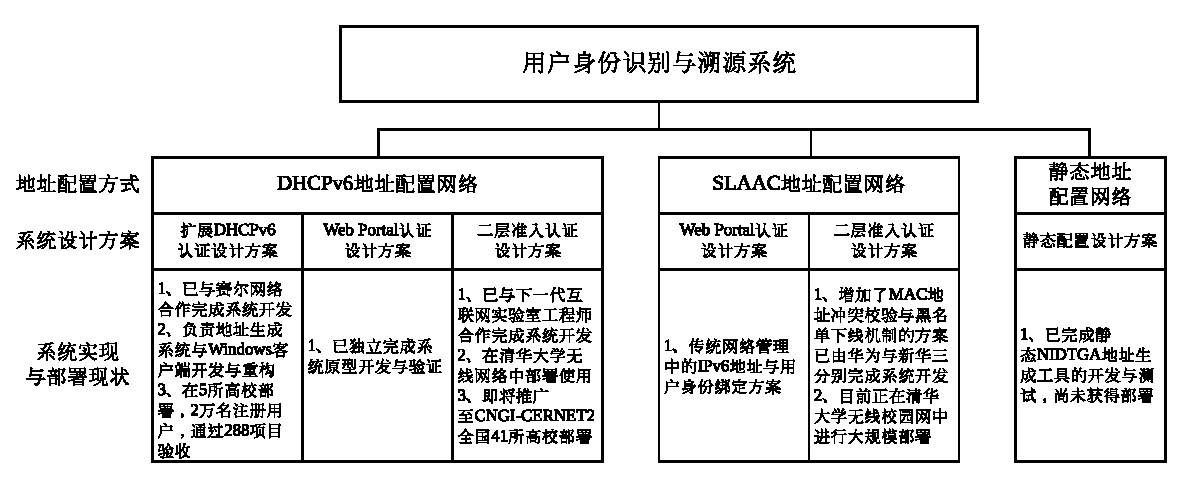
\includegraphics[width=\textwidth]{system_implementation_status.pdf}
    \caption{用户身份识别与溯源系统各种设计方案实现与部署情况}
    \label{fig:system_implementation_status}
  \end{figure}
